\chapter{Additional Simulation results}
\label{appendix_MCresults}
Some simulation results were omitted from chapter~\ref{chapTB}, specifically response plots relating to the various physics lists. These have been included in this appendix.

\section{Results Obtained using Cylindrical Clusters}
Figures~\ref{TBplot_pion_response_4L_MC_QGSP} (\ref{TBplot_pion_response_4H_MC_QGSP}), \ref{TBplot_pion_response_4L_MC_QGSPHP} (\ref{TBplot_pion_response_4H_MC_QGSPHP}), and \ref{TBplot_pion_response_4L_MC_FTFP} (\ref{TBplot_pion_response_4H_MC_FTFP}) show the responses obtained from beams of pions directed at position 4L (4H), for the QGSP\_BERT, QGSP\_BERT\_HP, and FTFP\_BERT physics lists, respectively. The simulation results are analysed using the same method as for data, that is, cylindrical clusters of radius 16 cm are formed around the beam impact point, and the clustered energy is calibrated to the hadronic scale using a simple flat-weighting method (described in Chapter~\ref{chapTB}). The weights used for the calibration are derived from data, at a beam energy of 200 GeV.


\begin{figure}[p]
\begin{center}
\subfigure{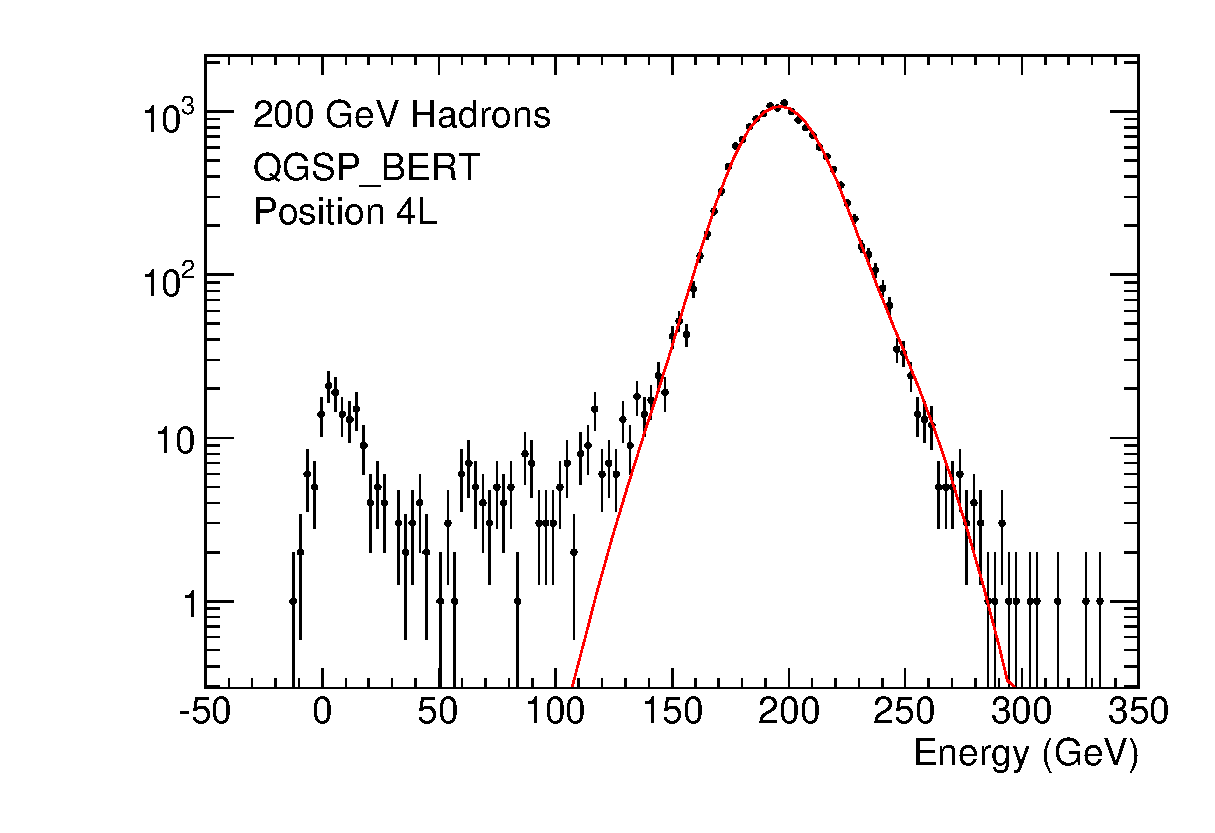
\includegraphics[width=0.45\linewidth,angle=0]{FCalTB_plots/Response_individual_MC/Pion_response_4L_200GeV_MC_QGSP.eps}}
\subfigure{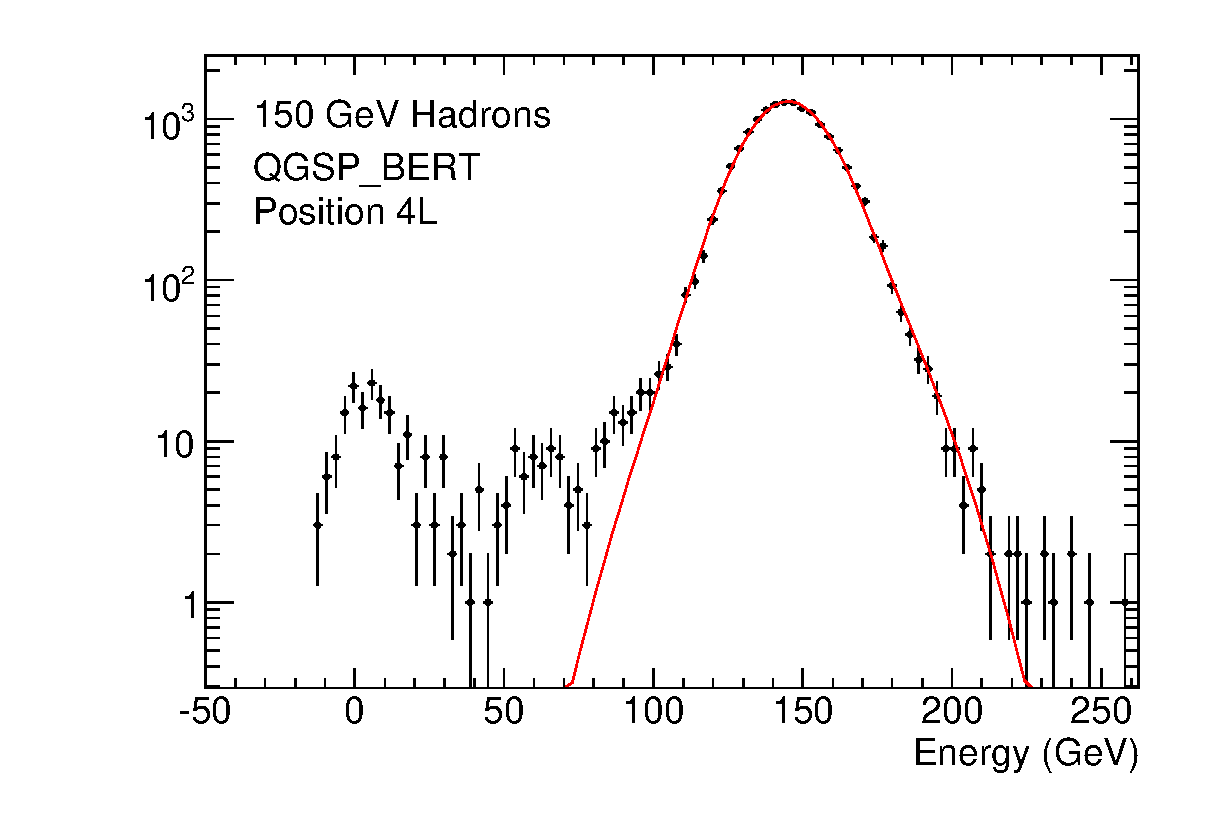
\includegraphics[width=0.45\linewidth,angle=0]{FCalTB_plots/Response_individual_MC/Pion_response_4L_150GeV_MC_QGSP.eps}}\\
\subfigure{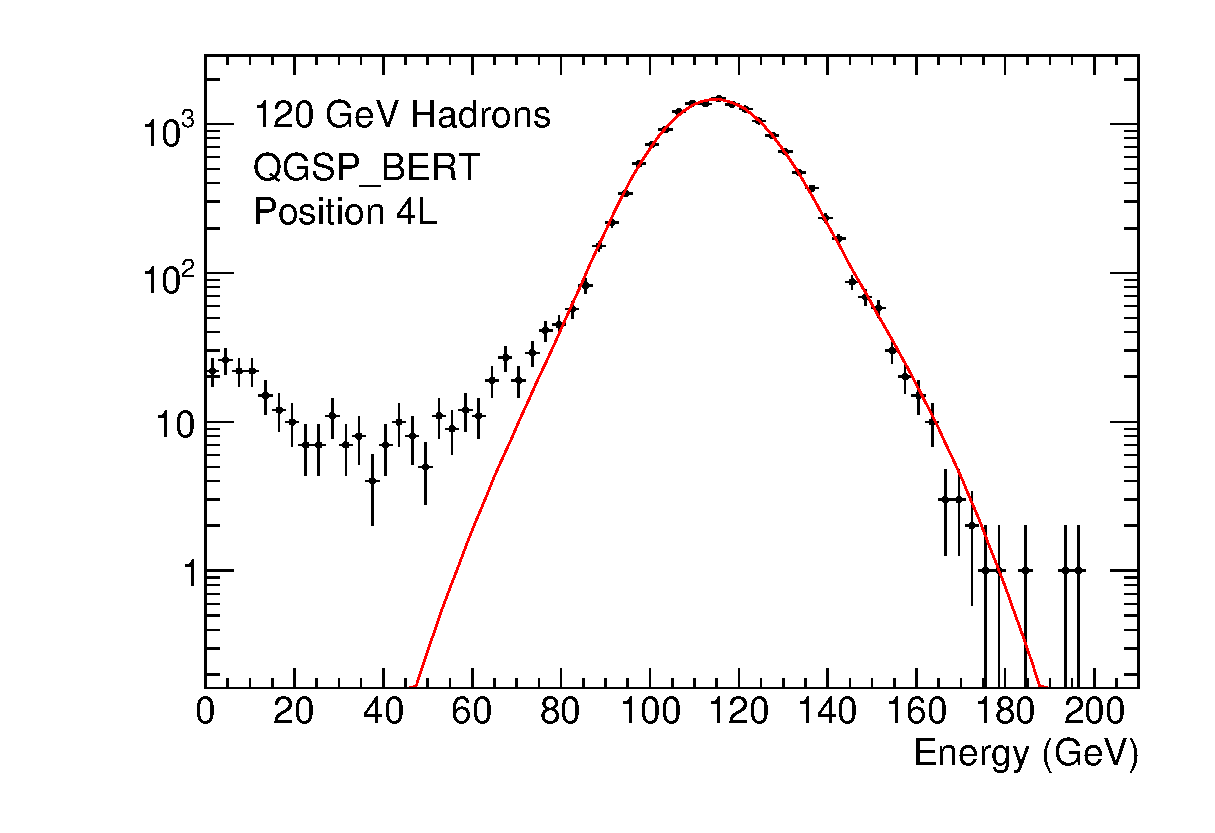
\includegraphics[width=0.45\linewidth,angle=0]{FCalTB_plots/Response_individual_MC/Pion_response_4L_120GeV_MC_QGSP.eps}}
\subfigure{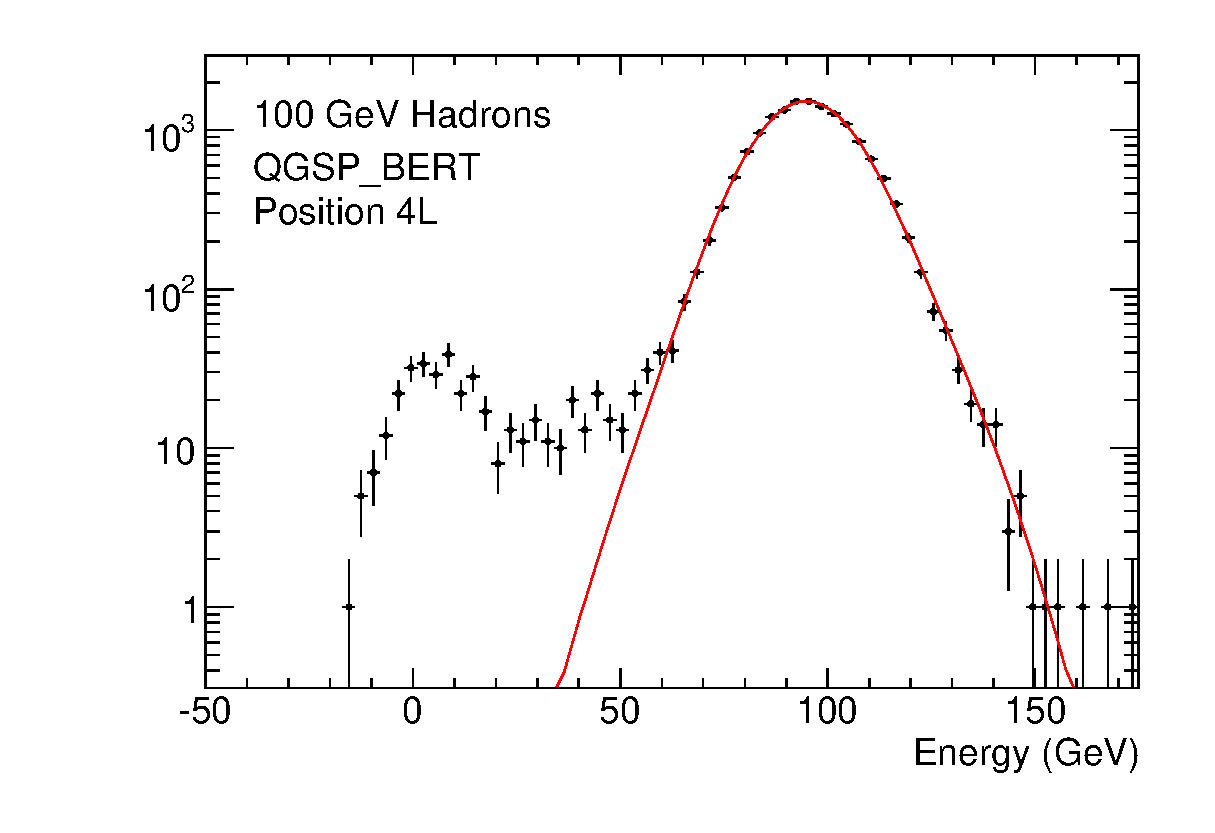
\includegraphics[width=0.45\linewidth,angle=0]{FCalTB_plots/Response_individual_MC/Pion_response_4L_100GeV_MC_QGSP.eps}}\\
\subfigure{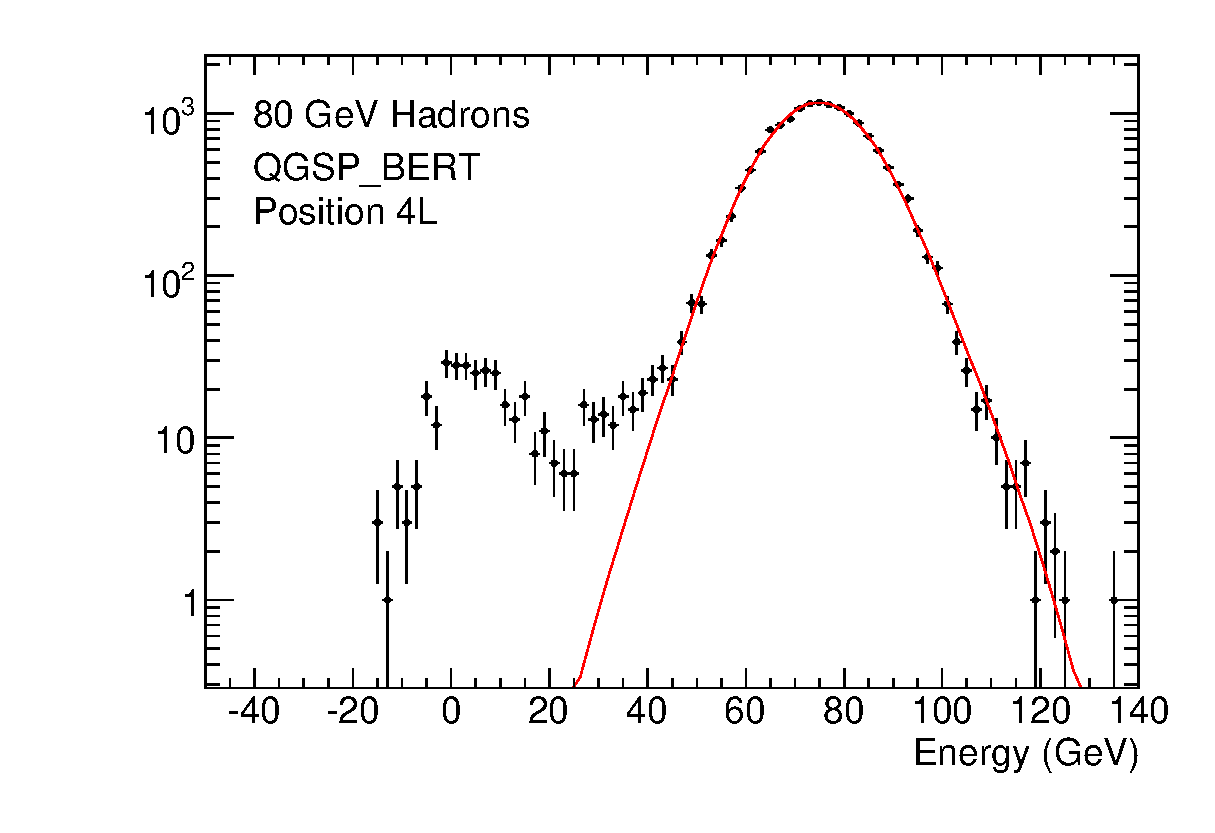
\includegraphics[width=0.45\linewidth,angle=0]{FCalTB_plots/Response_individual_MC/Pion_response_4L_80GeV_MC_QGSP.eps}}
\subfigure{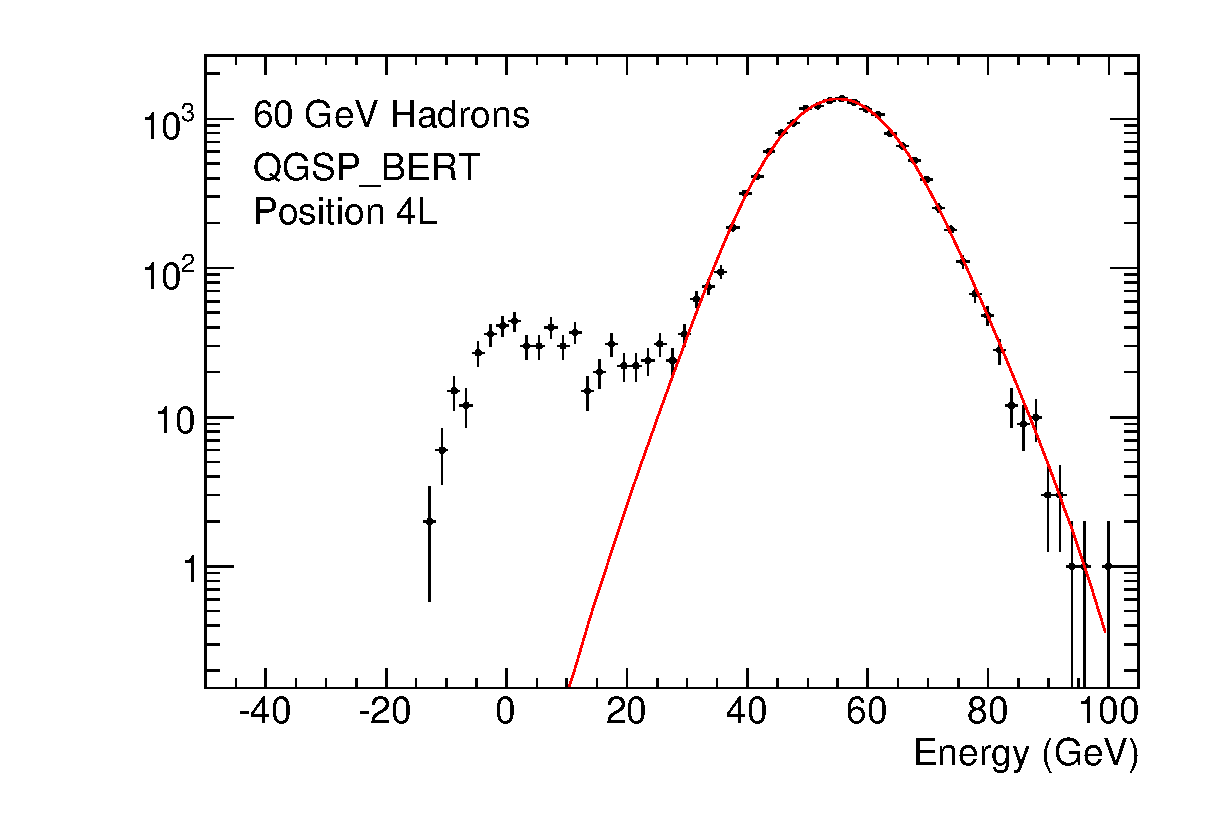
\includegraphics[width=0.45\linewidth,angle=0]{FCalTB_plots/Response_individual_MC/Pion_response_4L_60GeV_MC_QGSP.eps}}\\
\subfigure{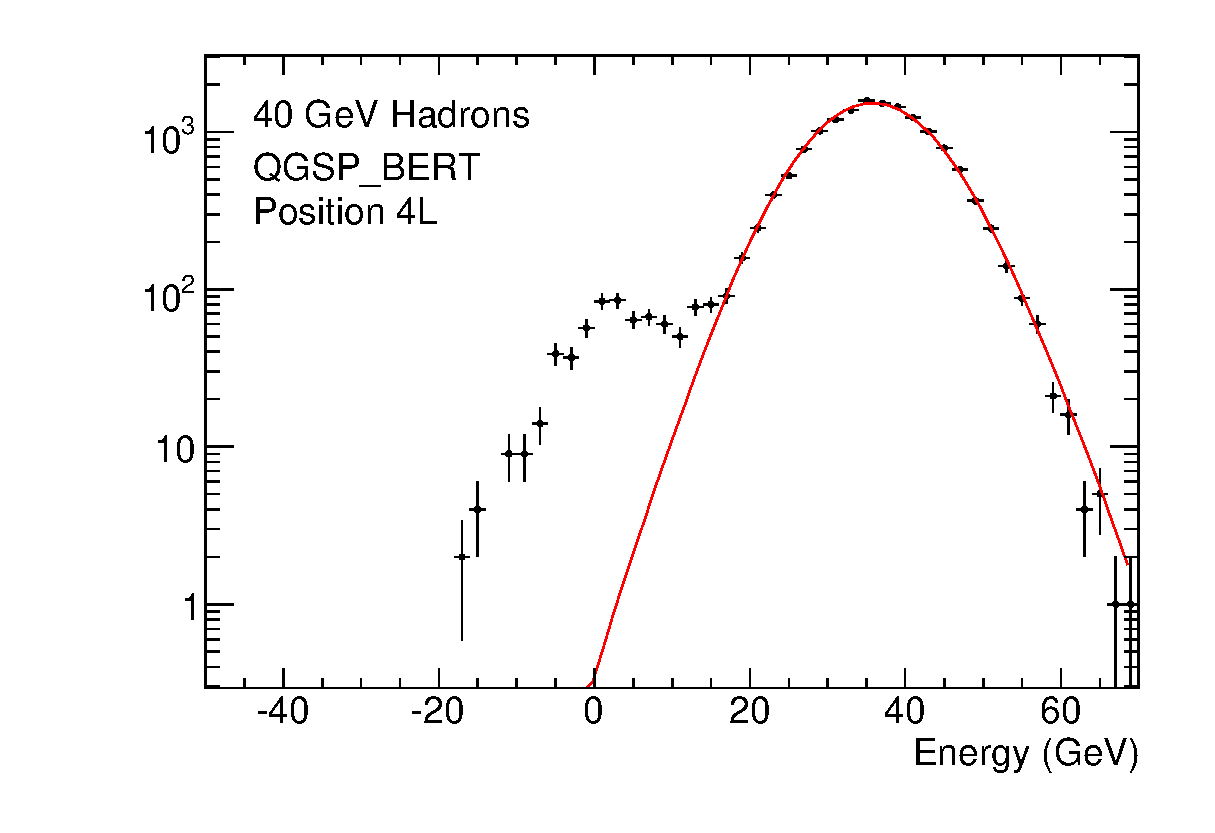
\includegraphics[width=0.45\linewidth,angle=0]{FCalTB_plots/Response_individual_MC/Pion_response_4L_40GeV_MC_QGSP.eps}}
\subfigure{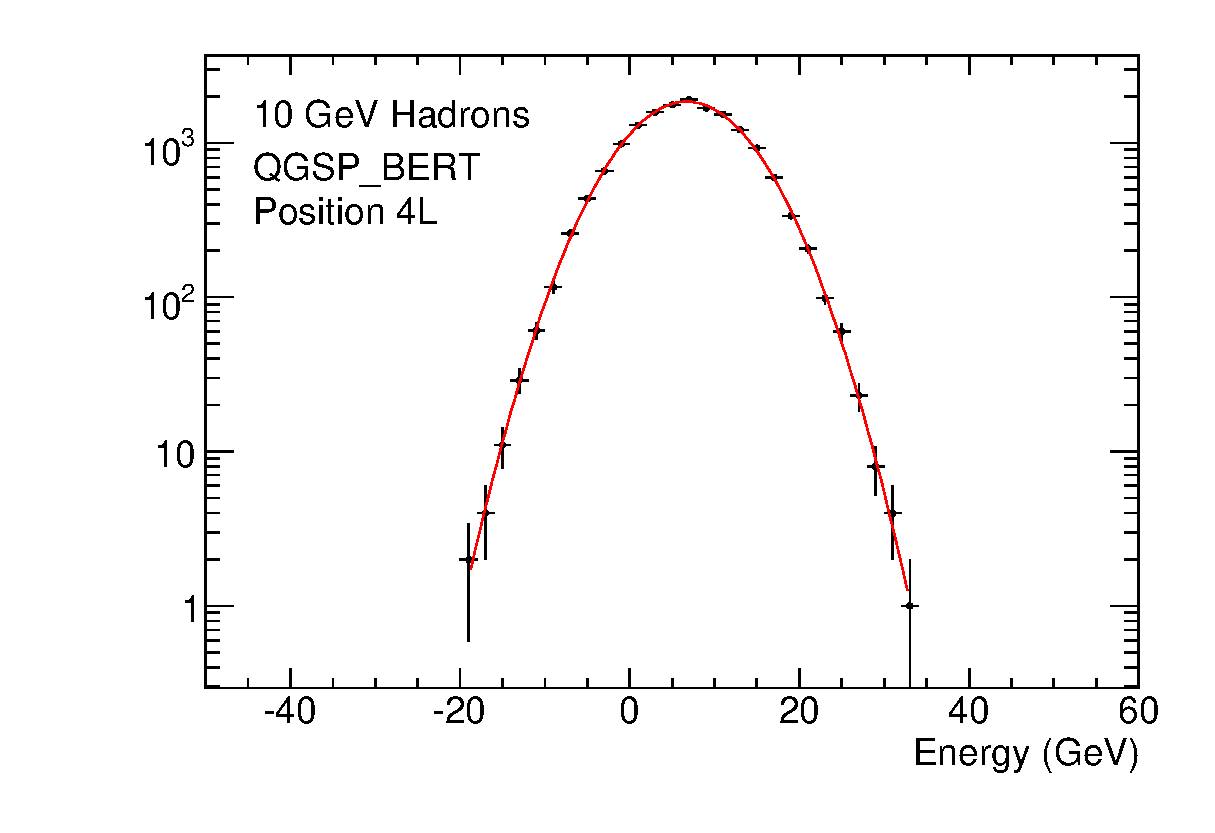
\includegraphics[width=0.45\linewidth,angle=0]{FCalTB_plots/Response_individual_MC/Pion_response_4L_10GeV_MC_QGSP.eps}}\\
\end{center}
\caption[Pions at 4L, QGSP\_BERT]{Response plots for pions directed at position 4L, simulated using the QGSP\_BERT physics list.}
\label{TBplot_pion_response_4L_MC_QGSP}
\end{figure}

\begin{figure}[p]
\begin{center}
\subfigure{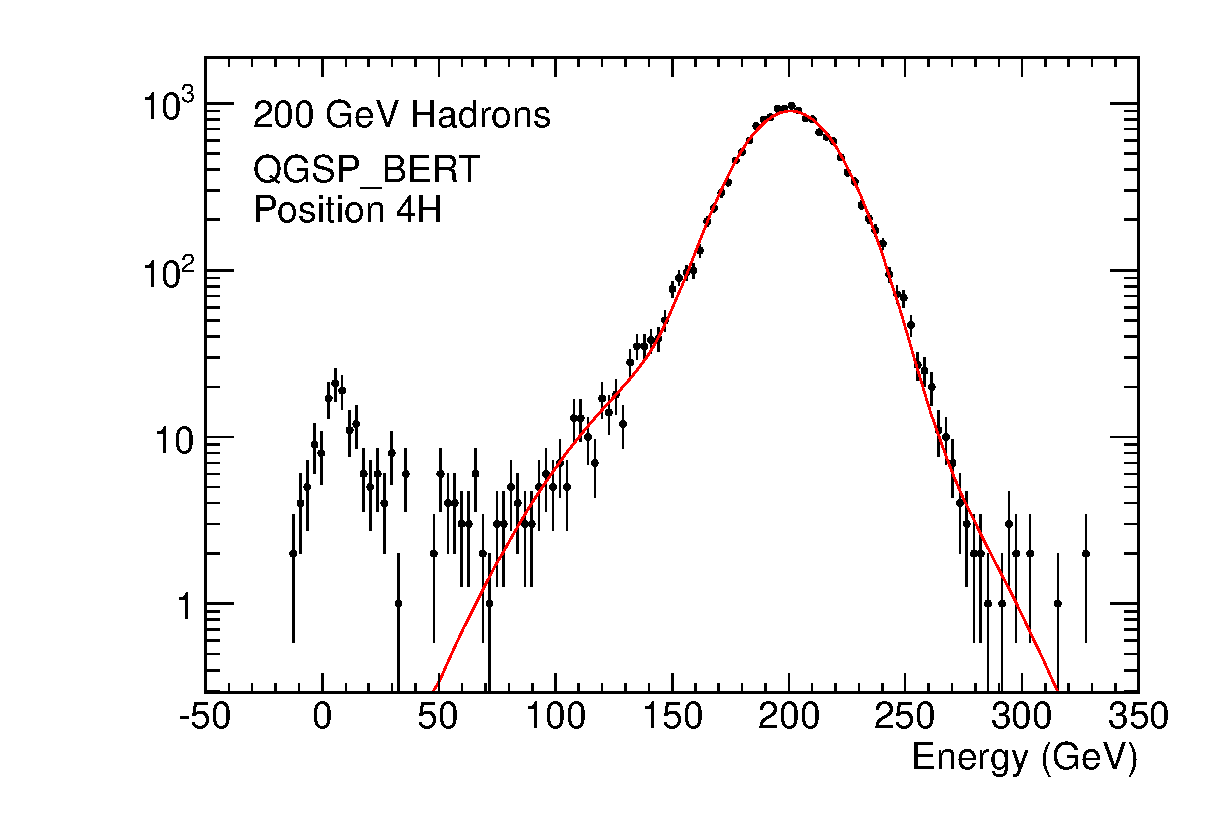
\includegraphics[width=0.45\linewidth,angle=0]{FCalTB_plots/Response_individual_MC/Pion_response_4H_200GeV_MC_QGSP.eps}}
\subfigure{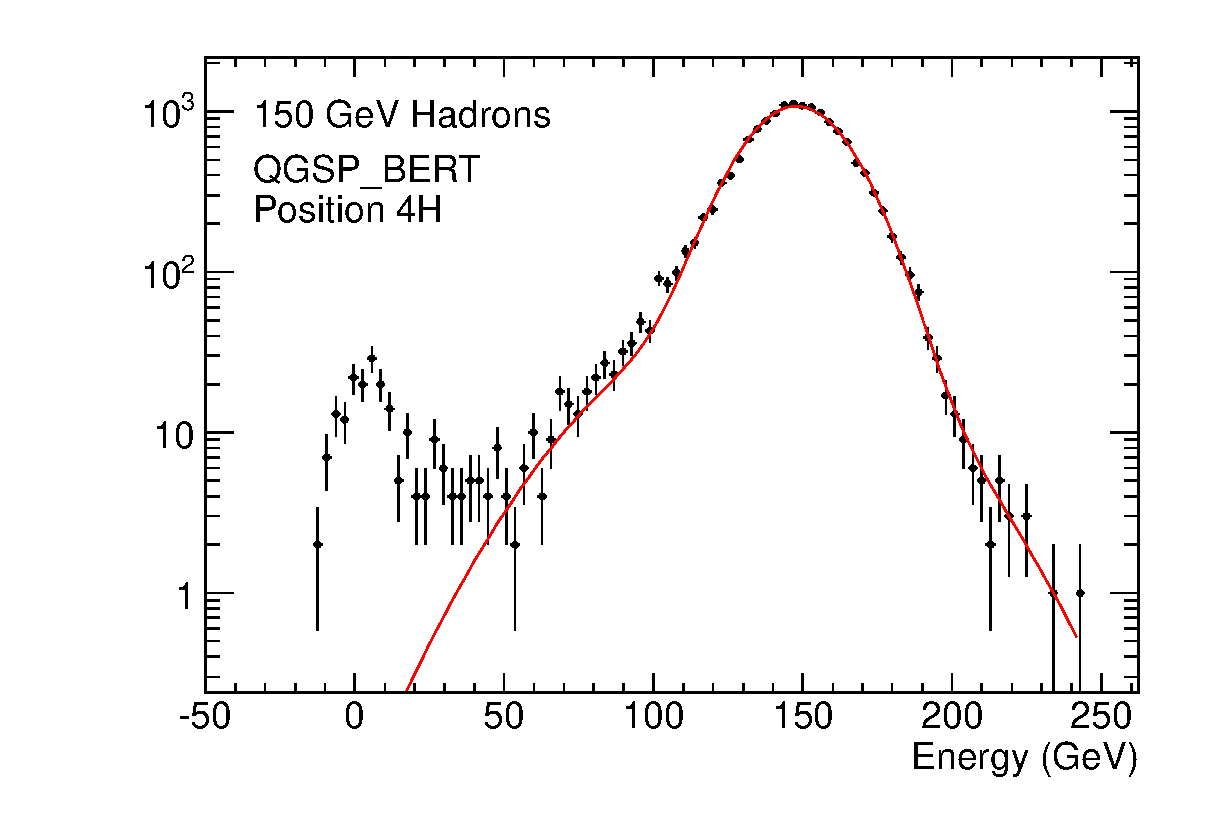
\includegraphics[width=0.45\linewidth,angle=0]{FCalTB_plots/Response_individual_MC/Pion_response_4H_150GeV_MC_QGSP.eps}}\\
\subfigure{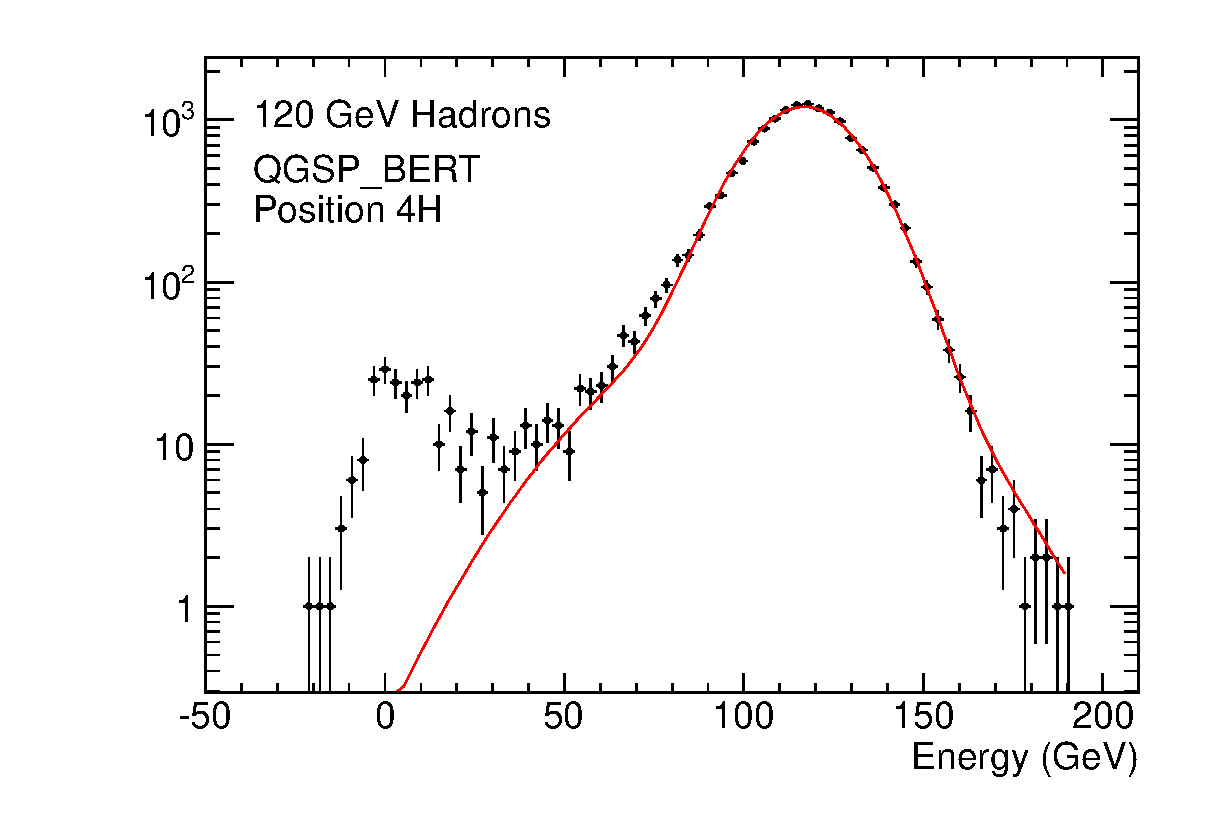
\includegraphics[width=0.45\linewidth,angle=0]{FCalTB_plots/Response_individual_MC/Pion_response_4H_120GeV_MC_QGSP.eps}}
\subfigure{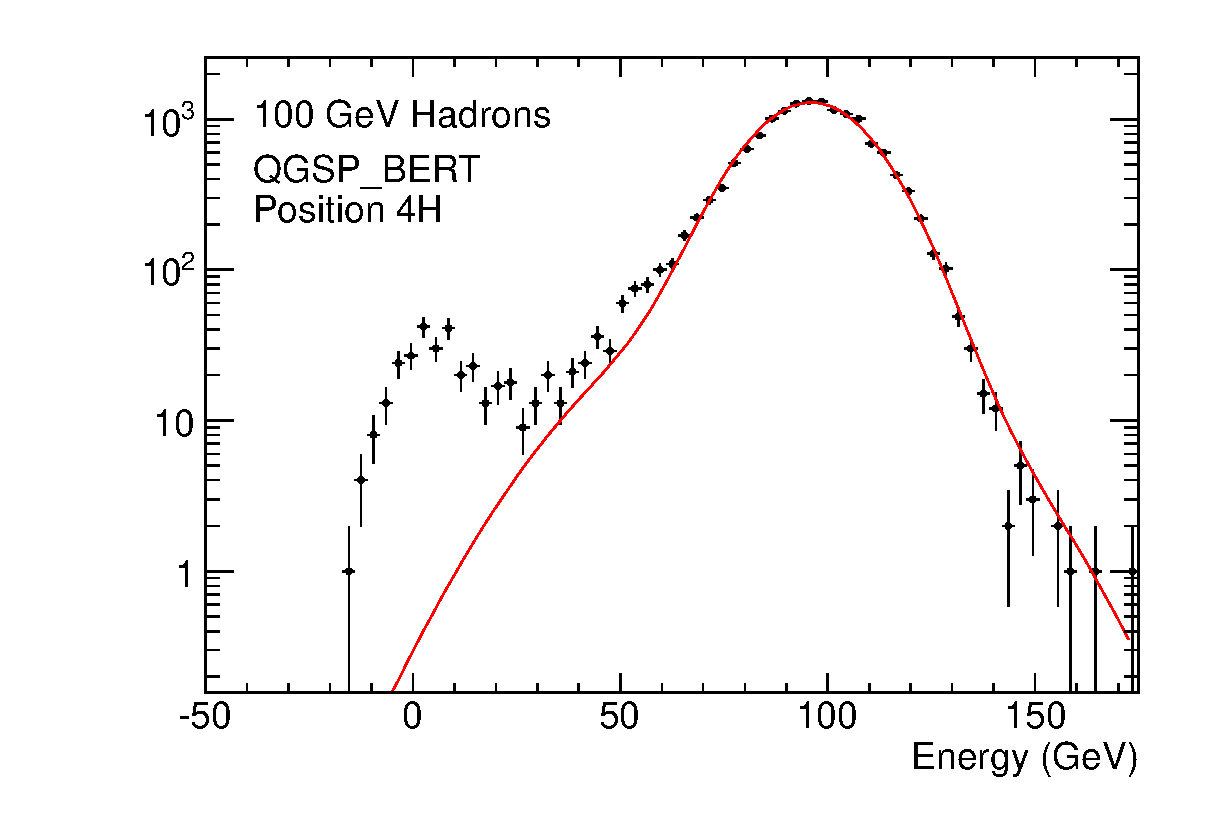
\includegraphics[width=0.45\linewidth,angle=0]{FCalTB_plots/Response_individual_MC/Pion_response_4H_100GeV_MC_QGSP.eps}}\\
\subfigure{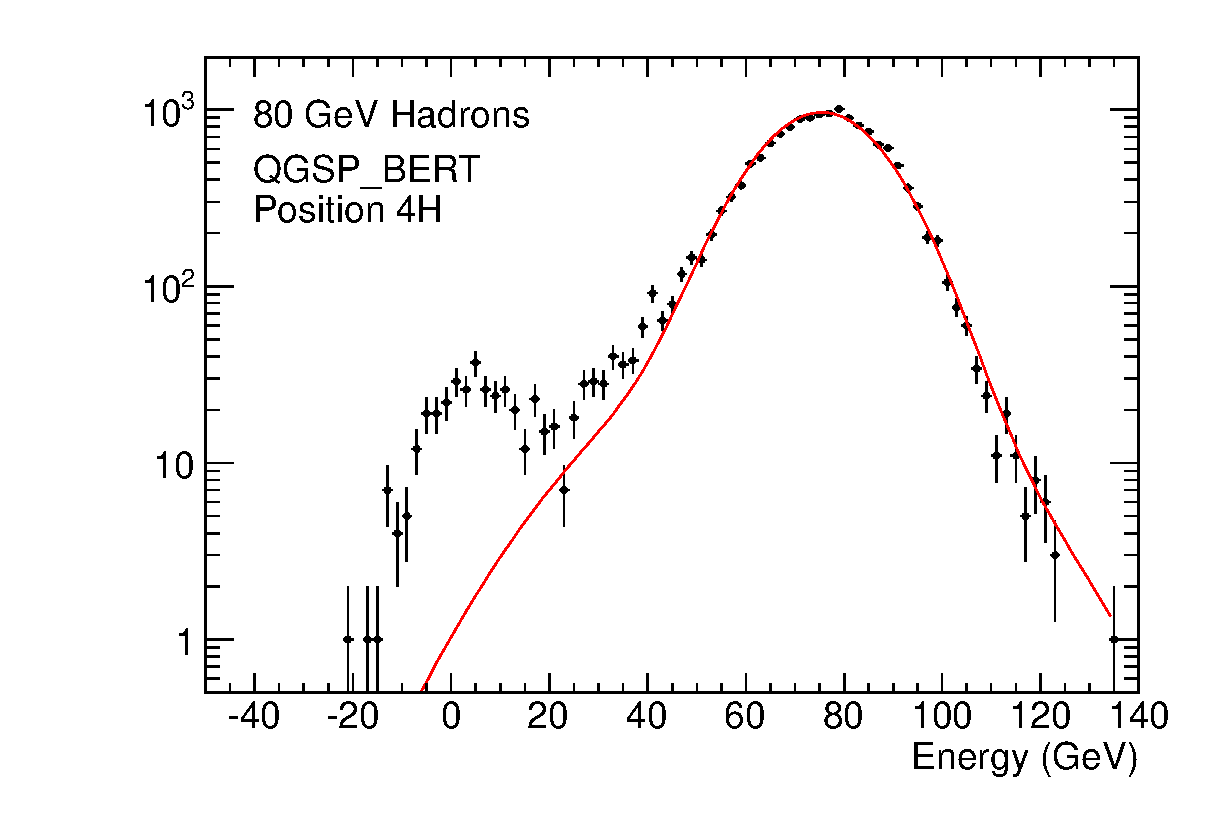
\includegraphics[width=0.45\linewidth,angle=0]{FCalTB_plots/Response_individual_MC/Pion_response_4H_80GeV_MC_QGSP.eps}}
\subfigure{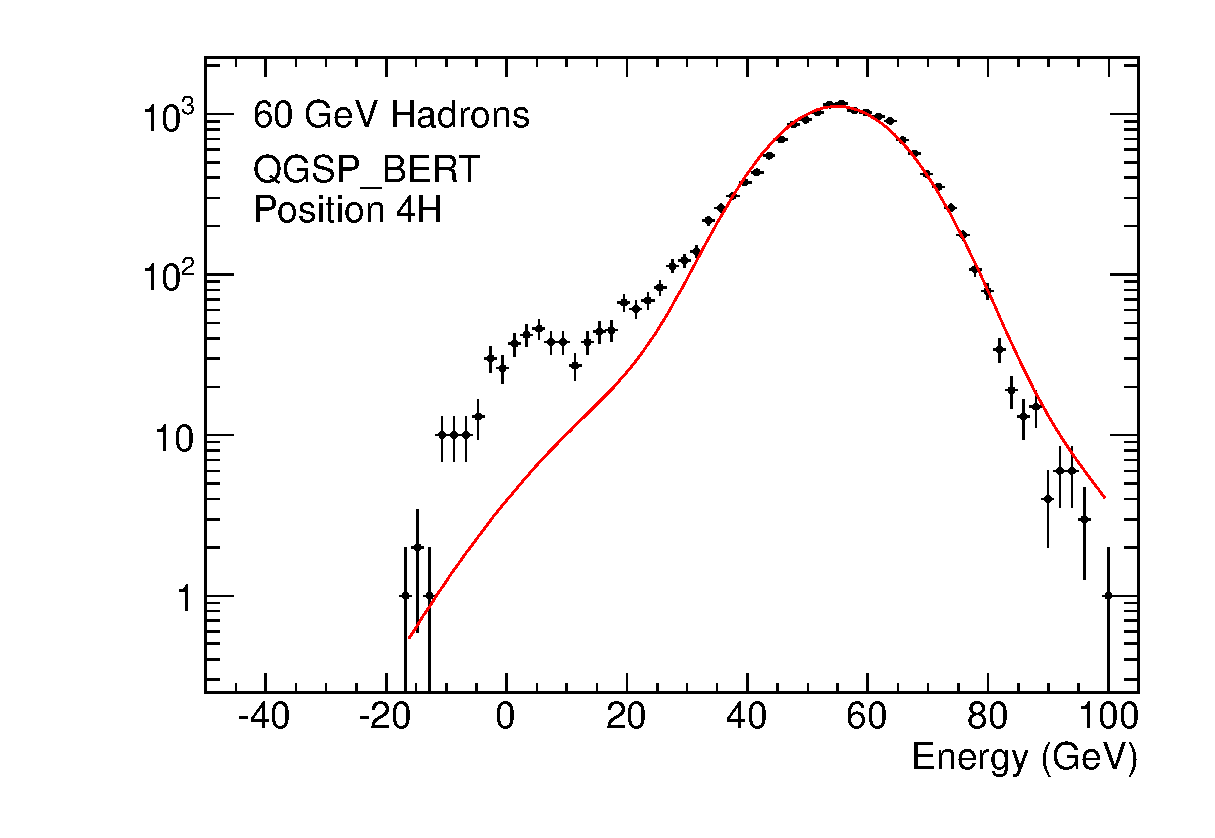
\includegraphics[width=0.45\linewidth,angle=0]{FCalTB_plots/Response_individual_MC/Pion_response_4H_60GeV_MC_QGSP.eps}}\\
\subfigure{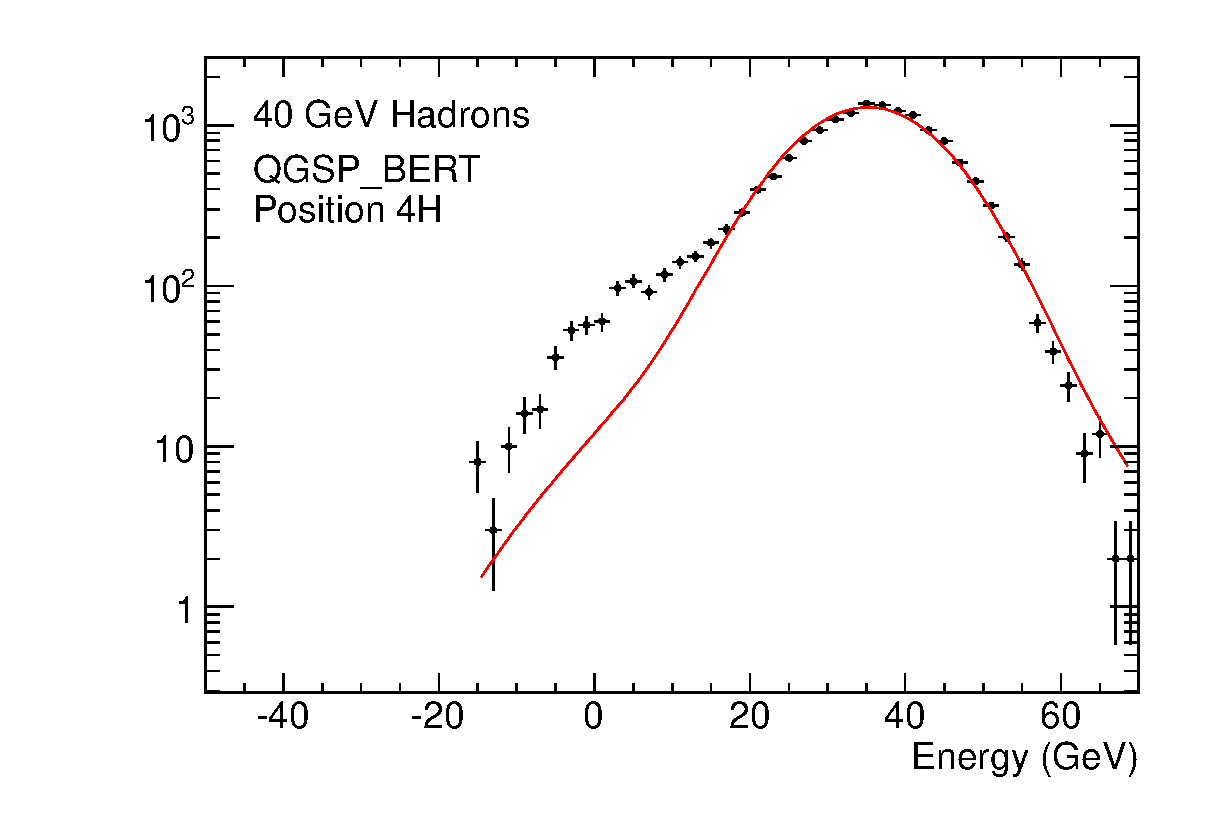
\includegraphics[width=0.45\linewidth,angle=0]{FCalTB_plots/Response_individual_MC/Pion_response_4H_40GeV_MC_QGSP.eps}}
\subfigure{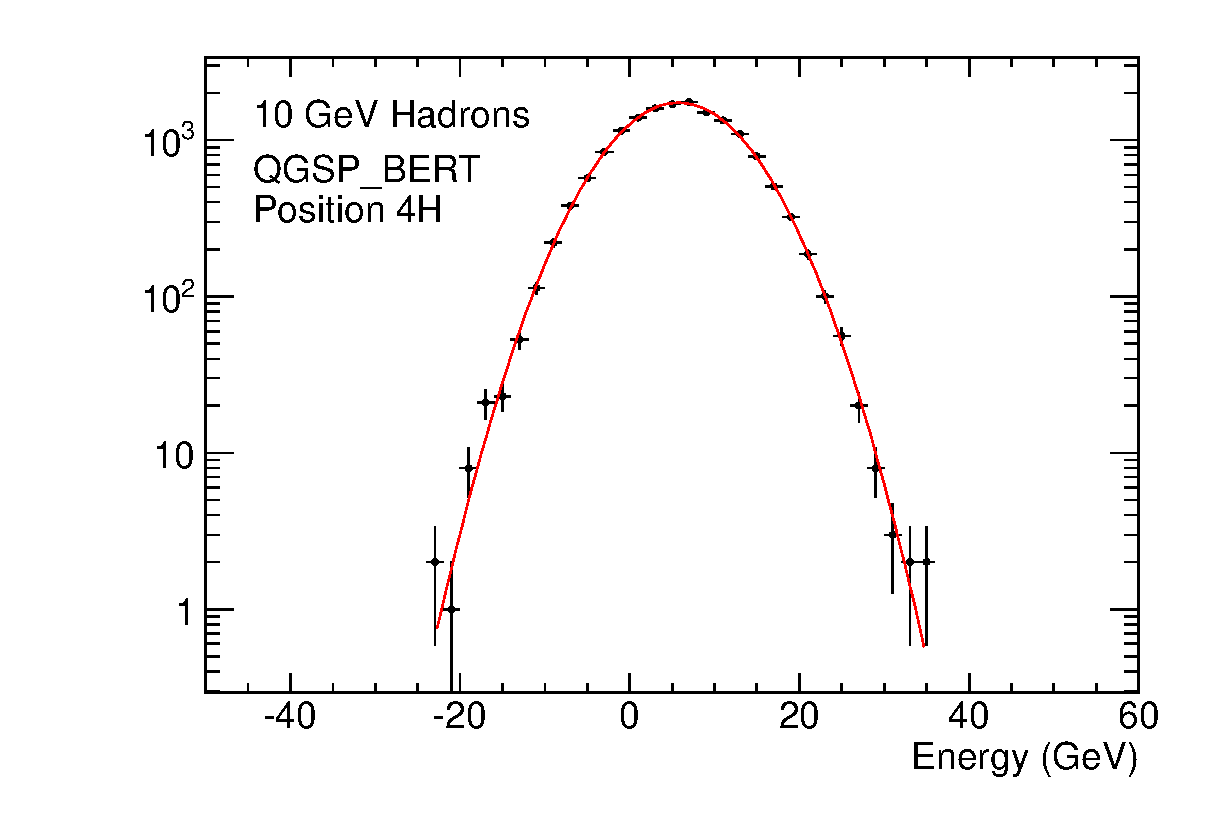
\includegraphics[width=0.45\linewidth,angle=0]{FCalTB_plots/Response_individual_MC/Pion_response_4H_10GeV_MC_QGSP.eps}}\\
\end{center}
\caption[Pions at 4H, QGSP\_BERT]{Response plots for pions directed at position 4H, simulated using the QGSP\_BERT physics list.}
\label{TBplot_pion_response_4H_MC_QGSP}
\end{figure}
%4H_MC table
%Resolution info:
%198.957 23.2254 14949 200.196 19.8853 15608.4 0.0075254 6.4724
%146.685 19.4212 14940.8 147.823 16.6907 15680.7 -0.0018378 6.60495
%115.733 17.0955 14886.1 116.795 14.9602 15589.9 0.0406184 7.20826
%95.2594 15.4311 14922.3 96.1448 14.0345 15653.2 0.0614355 7.52763
%74.7891 13.9024 15089.7 75.6103 12.6887 15788.7 -0.00961075 7.60855
%54.4073 11.9016 14901.2 55.2672 10.9448 15692.5 0.082152 6.95698
%34.8484 9.88262 14952.9 35.6385 9.28318 15785.8 0.0806734 6.48439
%5.75842 7.22804 15769 5.74872 7.28923 15703.9 -0.0170543 6.47252










\begin{figure}[p]
\begin{center}
\subfigure{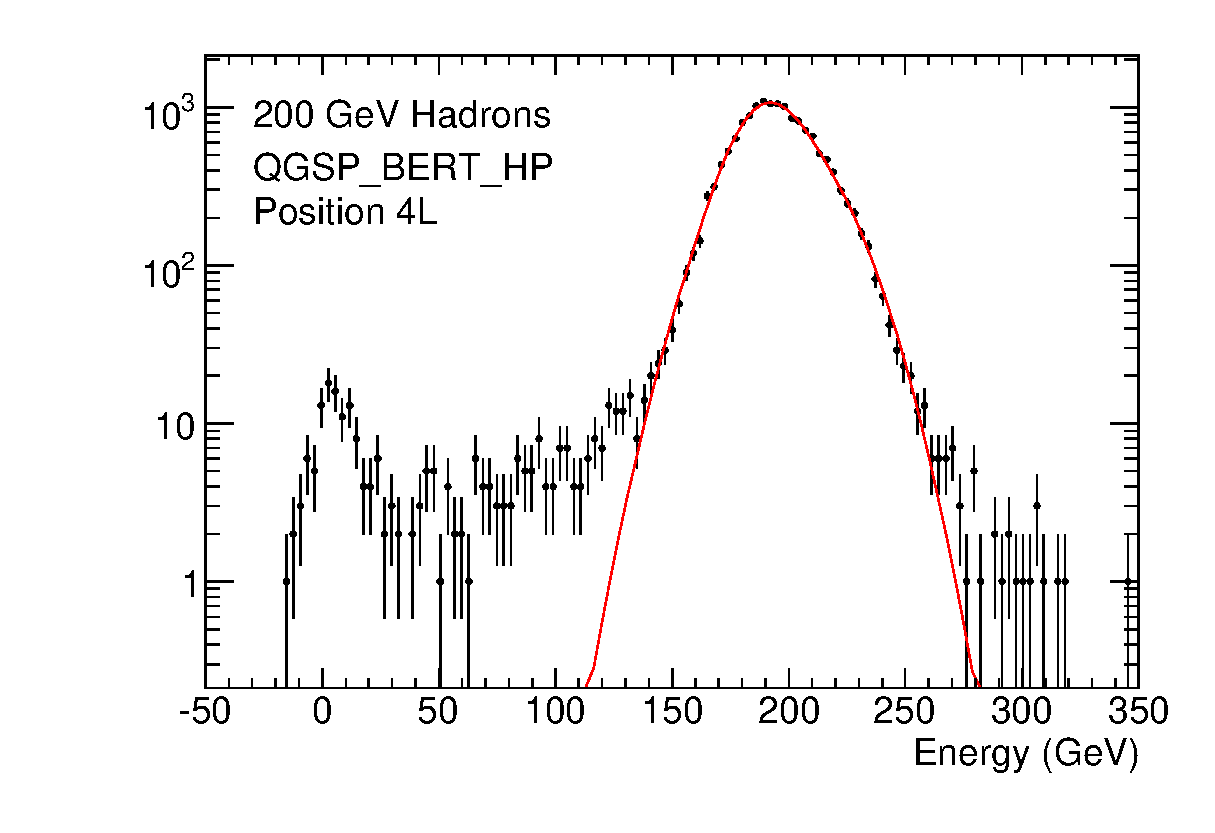
\includegraphics[width=0.45\linewidth,angle=0]{FCalTB_plots/Response_individual_MC/Pion_response_4L_200GeV_MC_QGSP_HP.eps}}
\subfigure{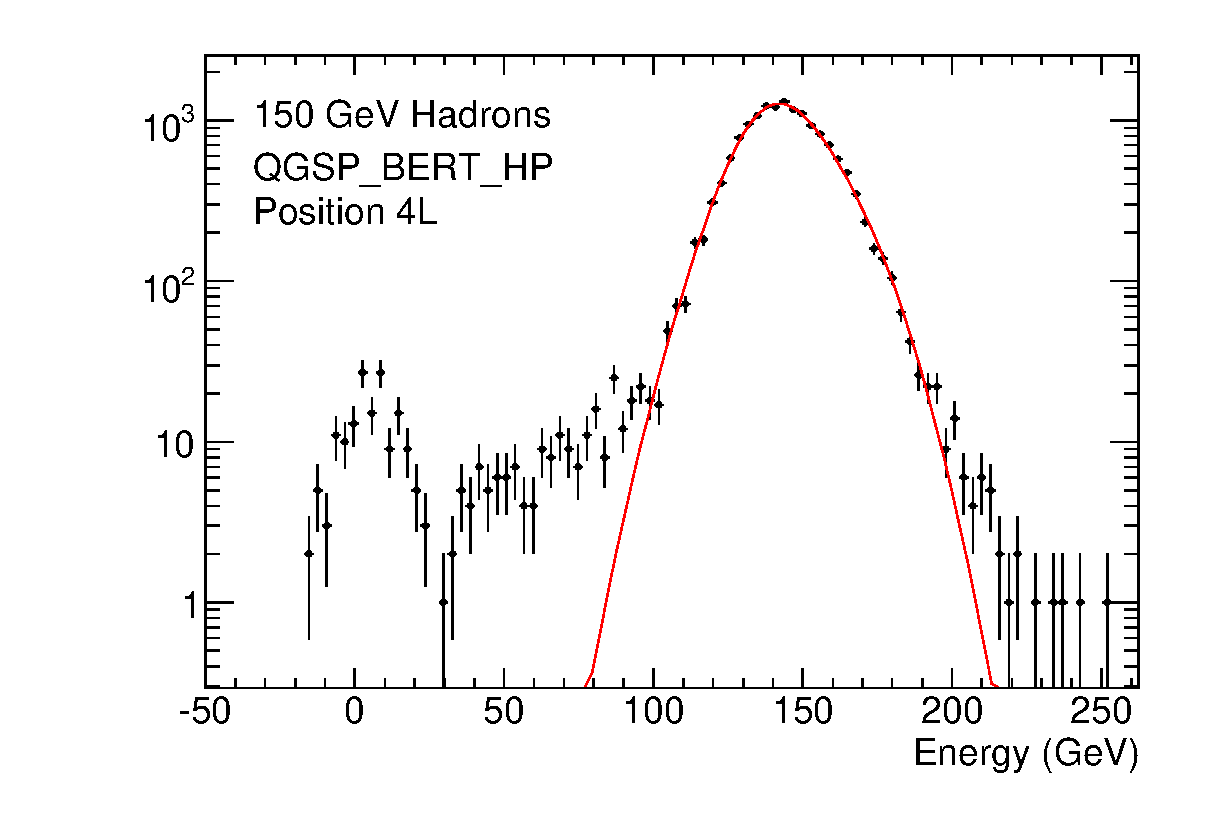
\includegraphics[width=0.45\linewidth,angle=0]{FCalTB_plots/Response_individual_MC/Pion_response_4L_150GeV_MC_QGSP_HP.eps}}\\
\subfigure{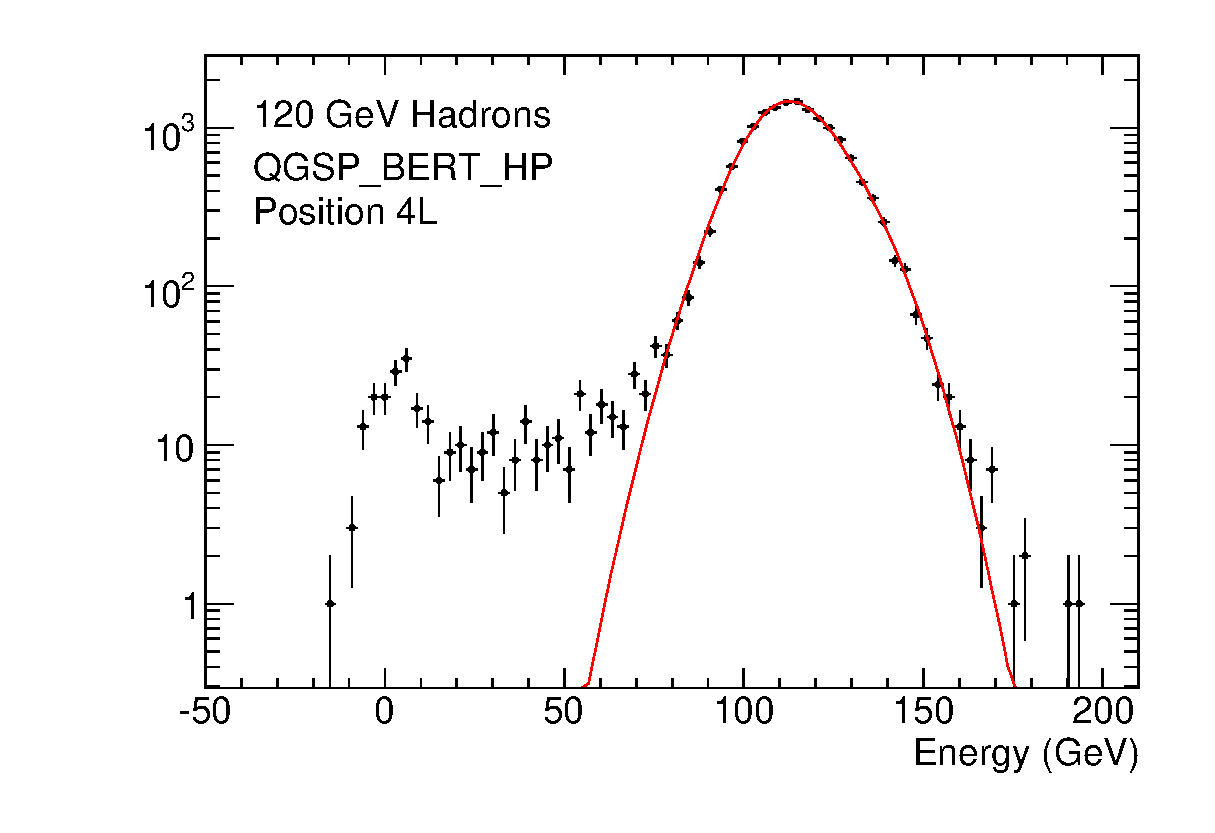
\includegraphics[width=0.45\linewidth,angle=0]{FCalTB_plots/Response_individual_MC/Pion_response_4L_120GeV_MC_QGSP_HP.eps}}
\subfigure{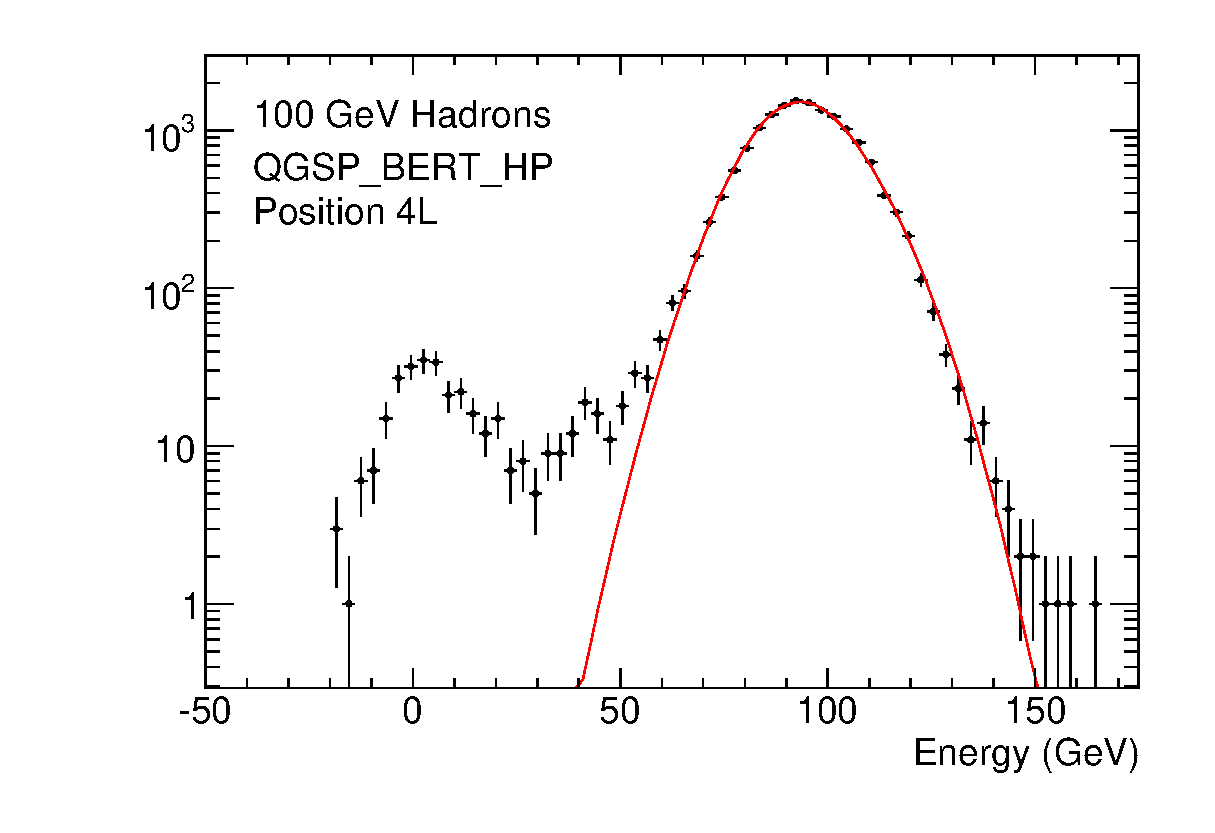
\includegraphics[width=0.45\linewidth,angle=0]{FCalTB_plots/Response_individual_MC/Pion_response_4L_100GeV_MC_QGSP_HP.eps}}\\
\subfigure{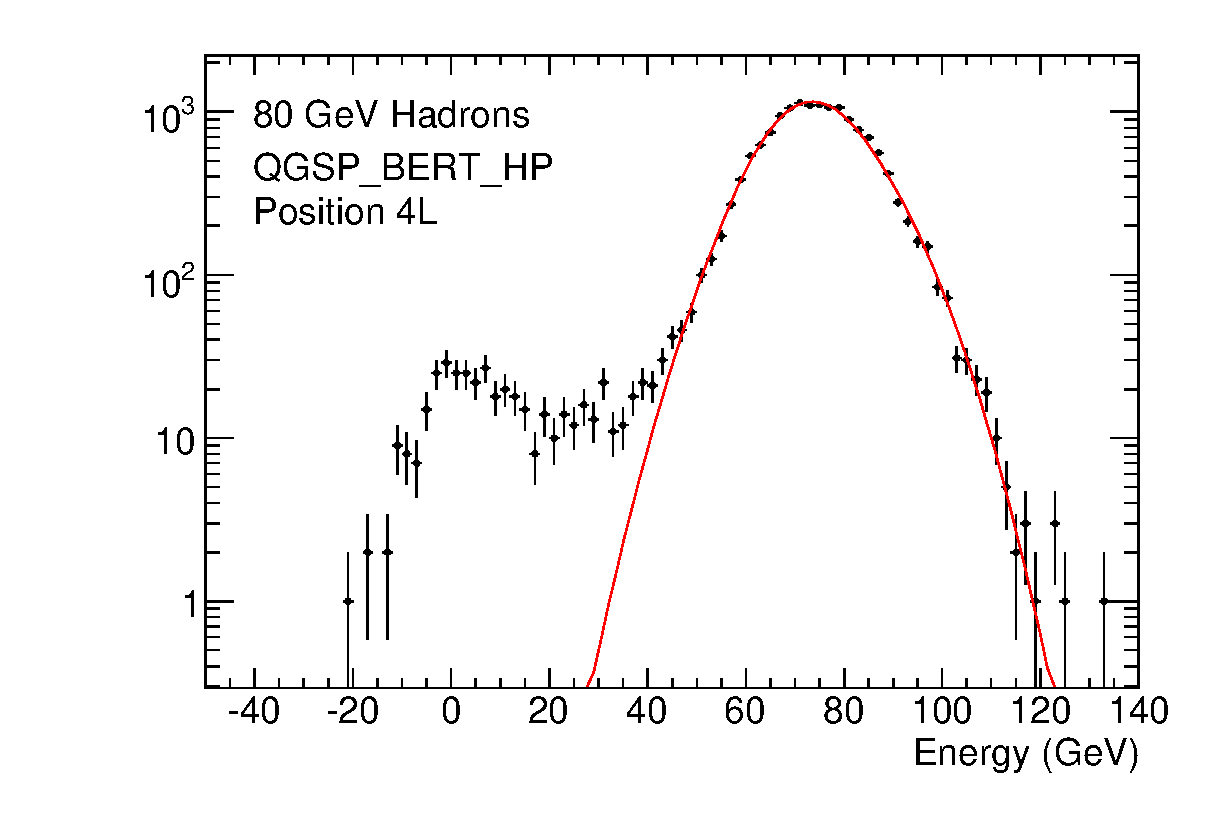
\includegraphics[width=0.45\linewidth,angle=0]{FCalTB_plots/Response_individual_MC/Pion_response_4L_80GeV_MC_QGSP_HP.eps}}
\subfigure{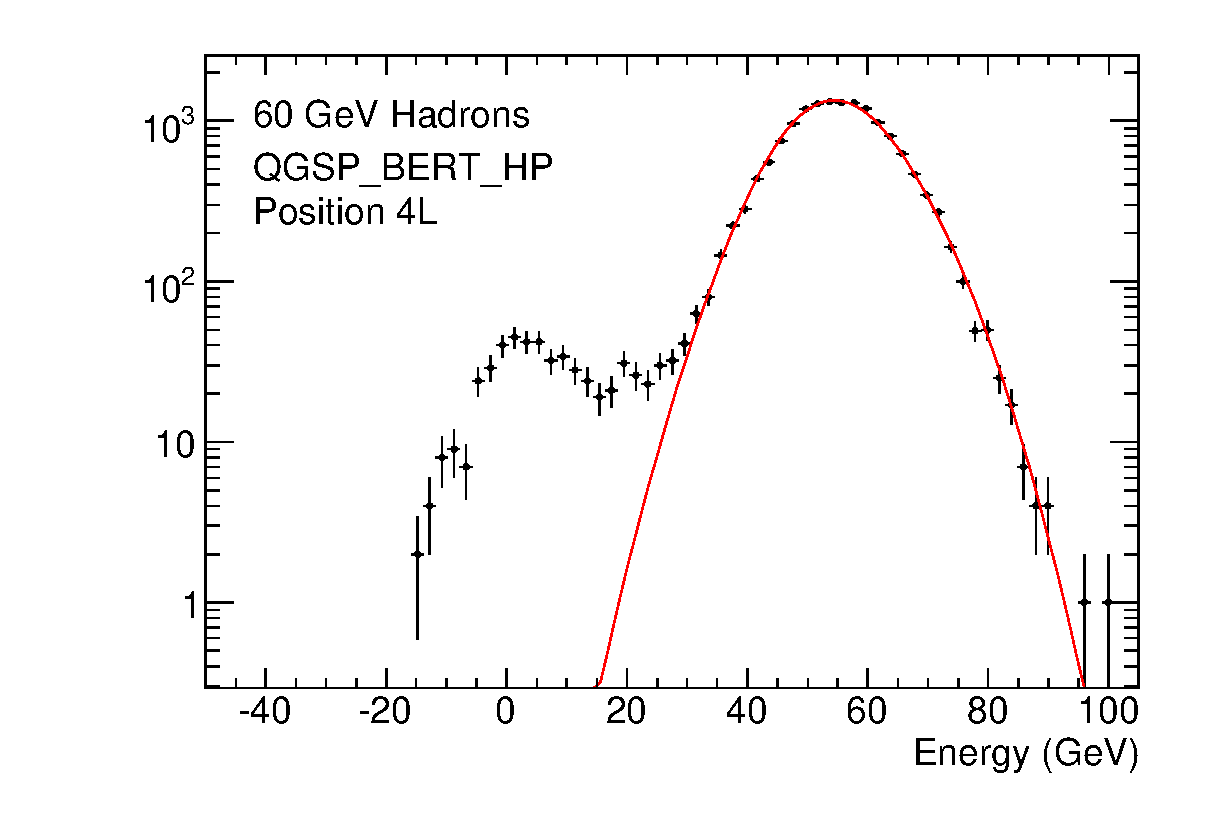
\includegraphics[width=0.45\linewidth,angle=0]{FCalTB_plots/Response_individual_MC/Pion_response_4L_60GeV_MC_QGSP_HP.eps}}\\
\subfigure{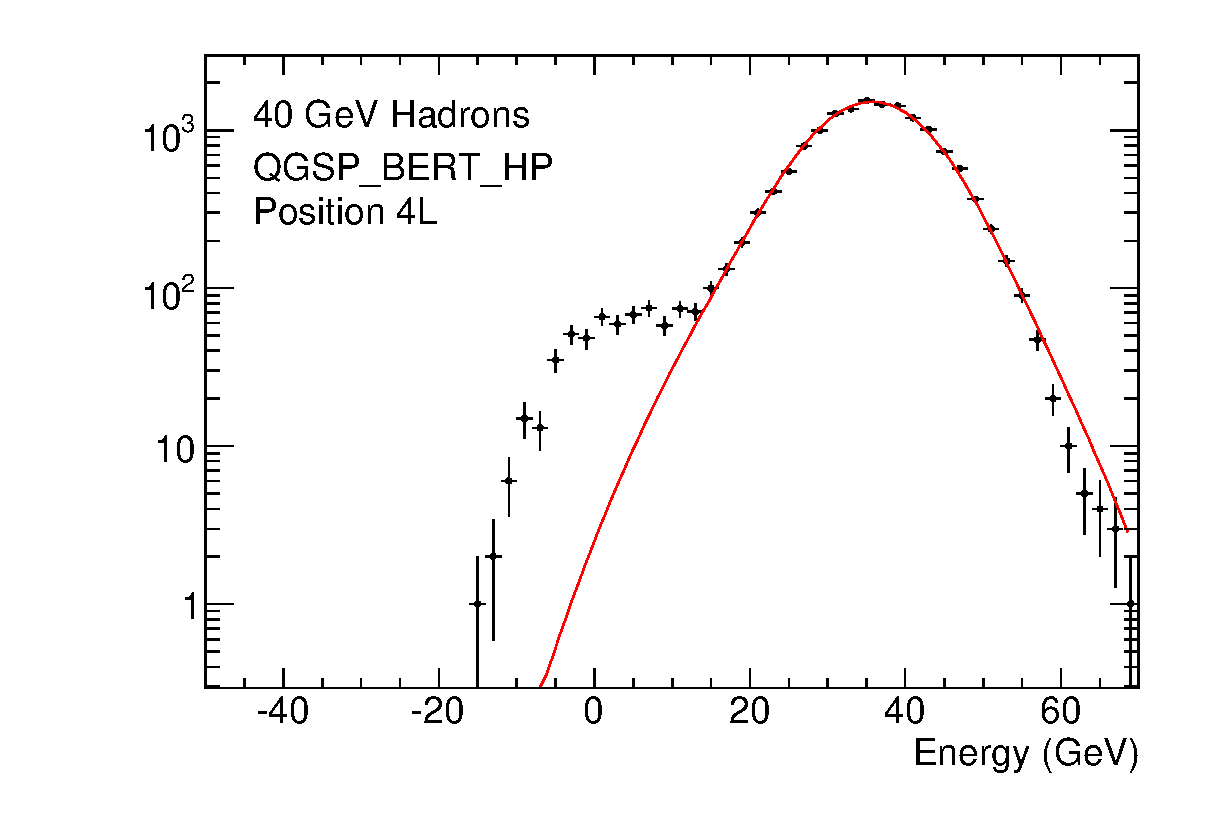
\includegraphics[width=0.45\linewidth,angle=0]{FCalTB_plots/Response_individual_MC/Pion_response_4L_40GeV_MC_QGSP_HP.eps}}
\subfigure{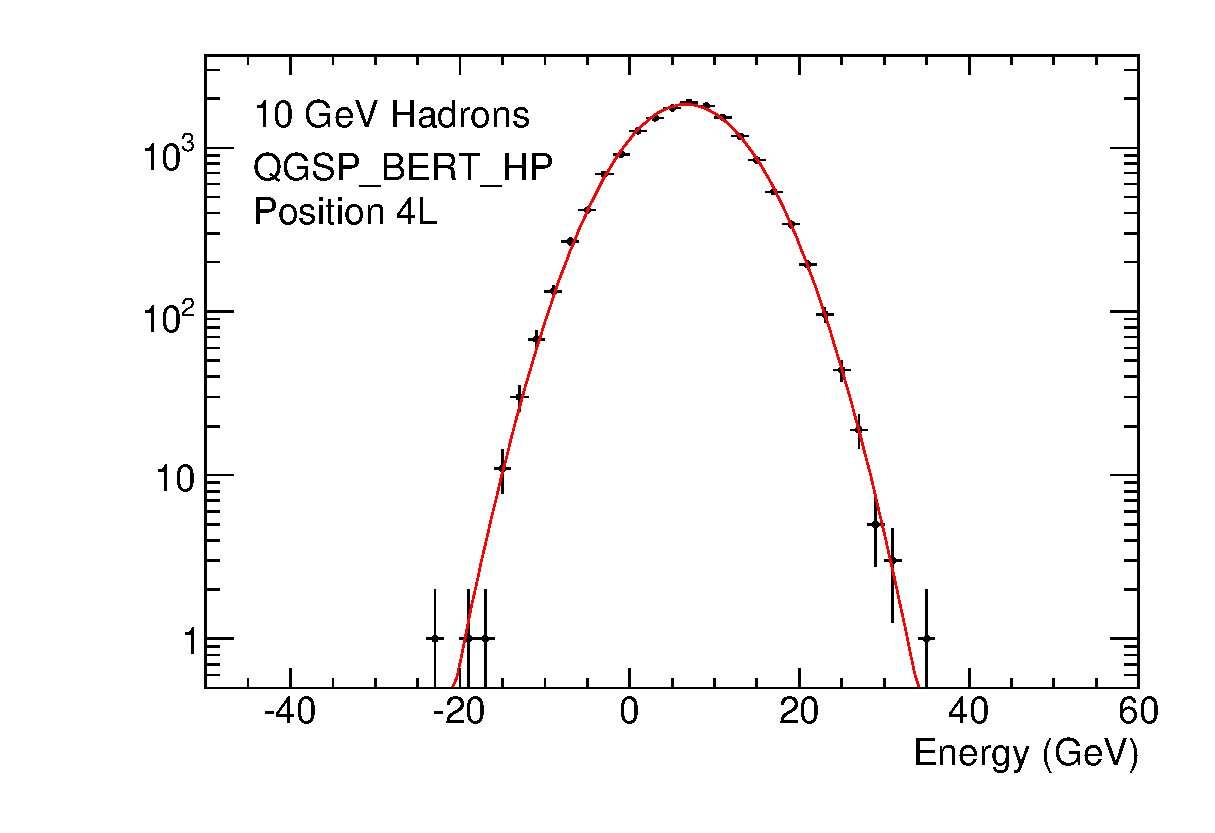
\includegraphics[width=0.45\linewidth,angle=0]{FCalTB_plots/Response_individual_MC/Pion_response_4L_10GeV_MC_QGSP_HP.eps}}\\
\end{center}
\caption[Pions at 4L, QGSP\_BERT\_HP]{Response plots for pions directed at position 4L, simulated using the QGSP\_BERT\_HP physics list.}
\label{TBplot_pion_response_4L_MC_QGSPHP}
\end{figure}

\begin{figure}[p]
\begin{center}
\subfigure{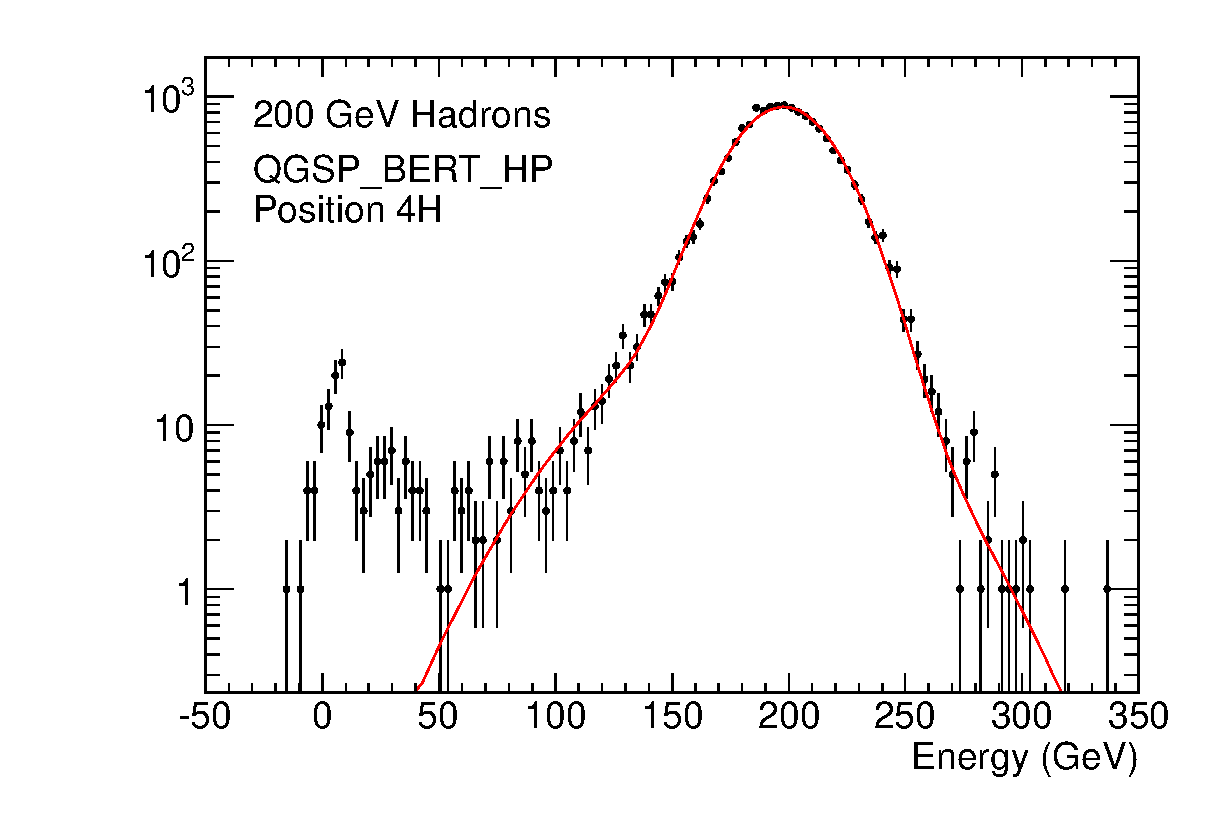
\includegraphics[width=0.45\linewidth,angle=0]{FCalTB_plots/Response_individual_MC/Pion_response_4H_200GeV_MC_QGSP_HP.eps}}
\subfigure{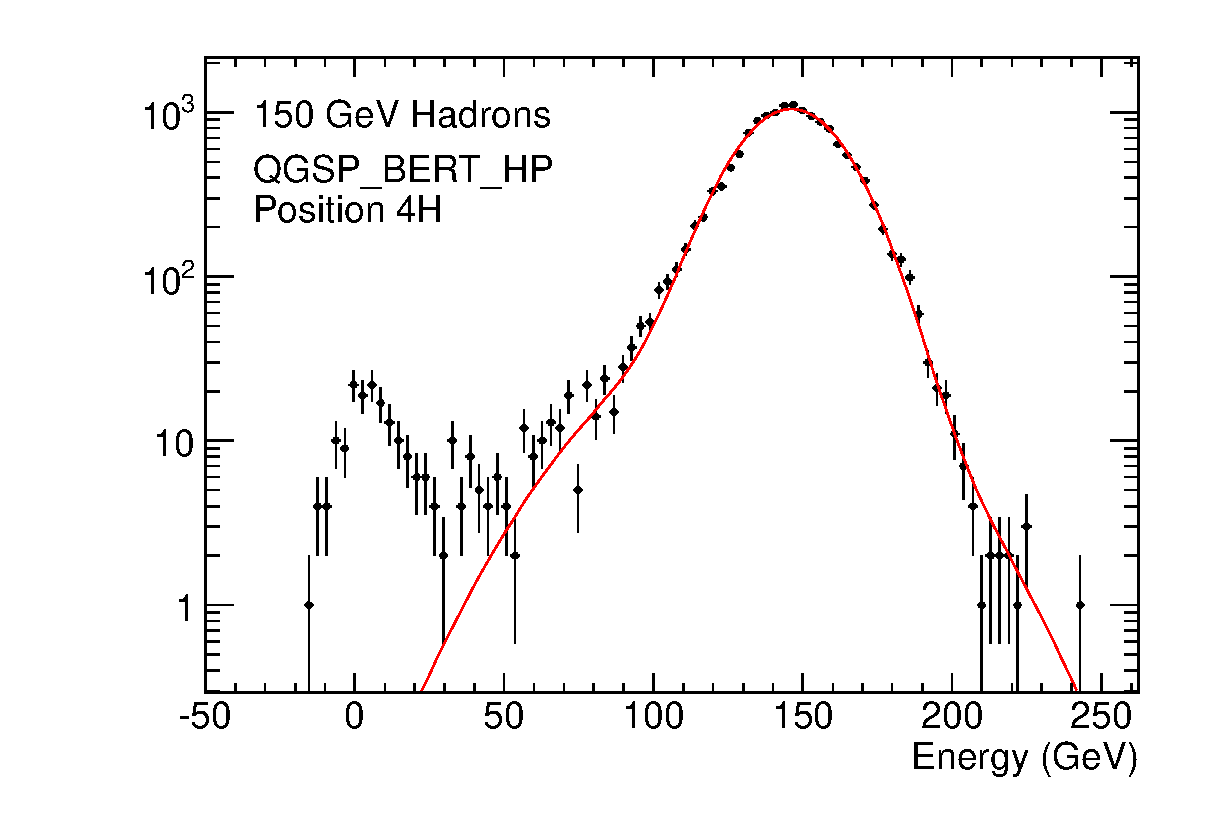
\includegraphics[width=0.45\linewidth,angle=0]{FCalTB_plots/Response_individual_MC/Pion_response_4H_150GeV_MC_QGSP_HP.eps}}\\
\subfigure{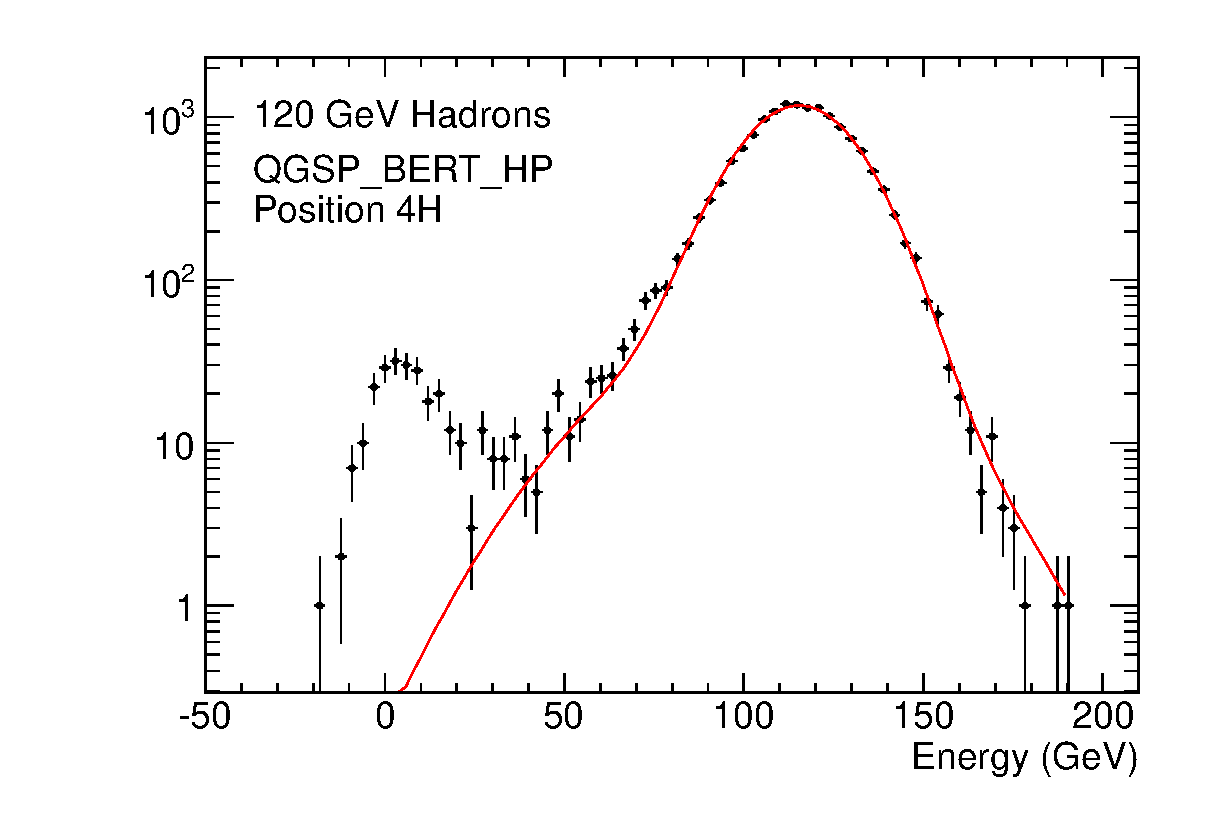
\includegraphics[width=0.45\linewidth,angle=0]{FCalTB_plots/Response_individual_MC/Pion_response_4H_120GeV_MC_QGSP_HP.eps}}
\subfigure{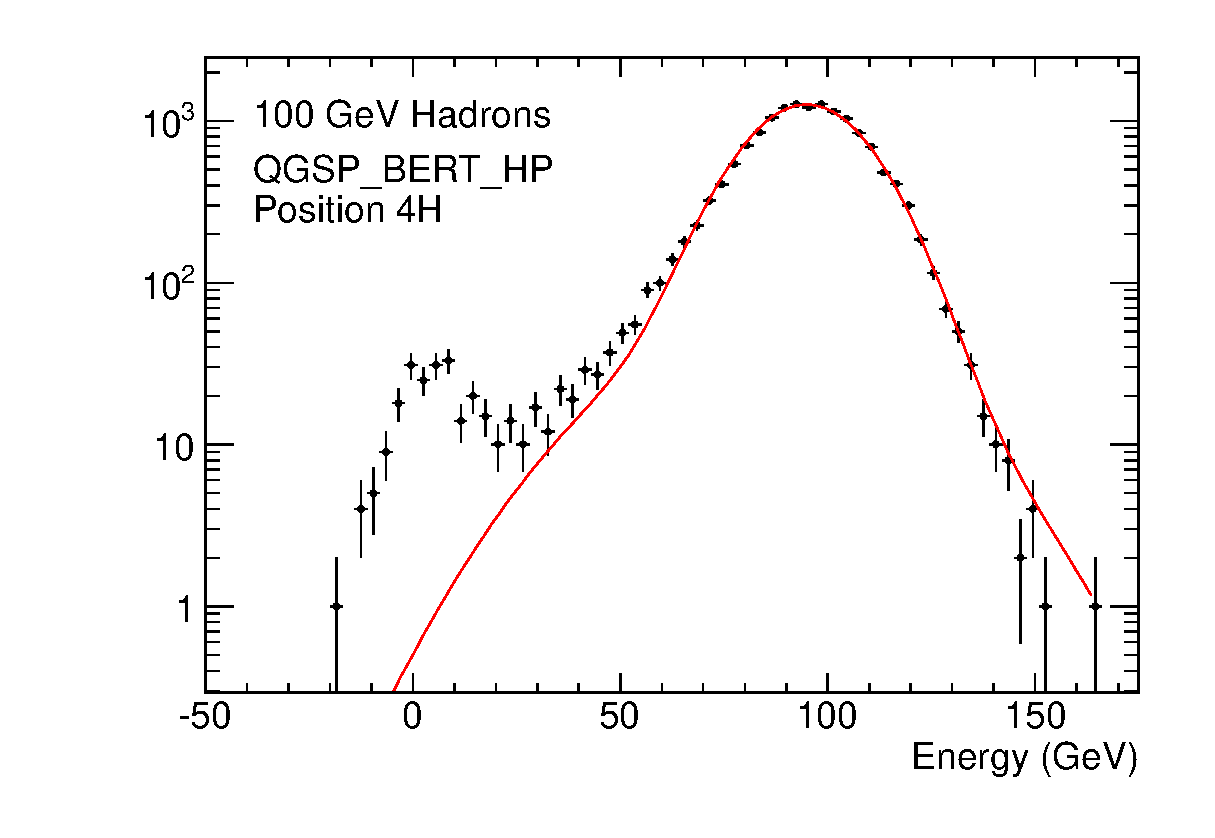
\includegraphics[width=0.45\linewidth,angle=0]{FCalTB_plots/Response_individual_MC/Pion_response_4H_100GeV_MC_QGSP_HP.eps}}\\
\subfigure{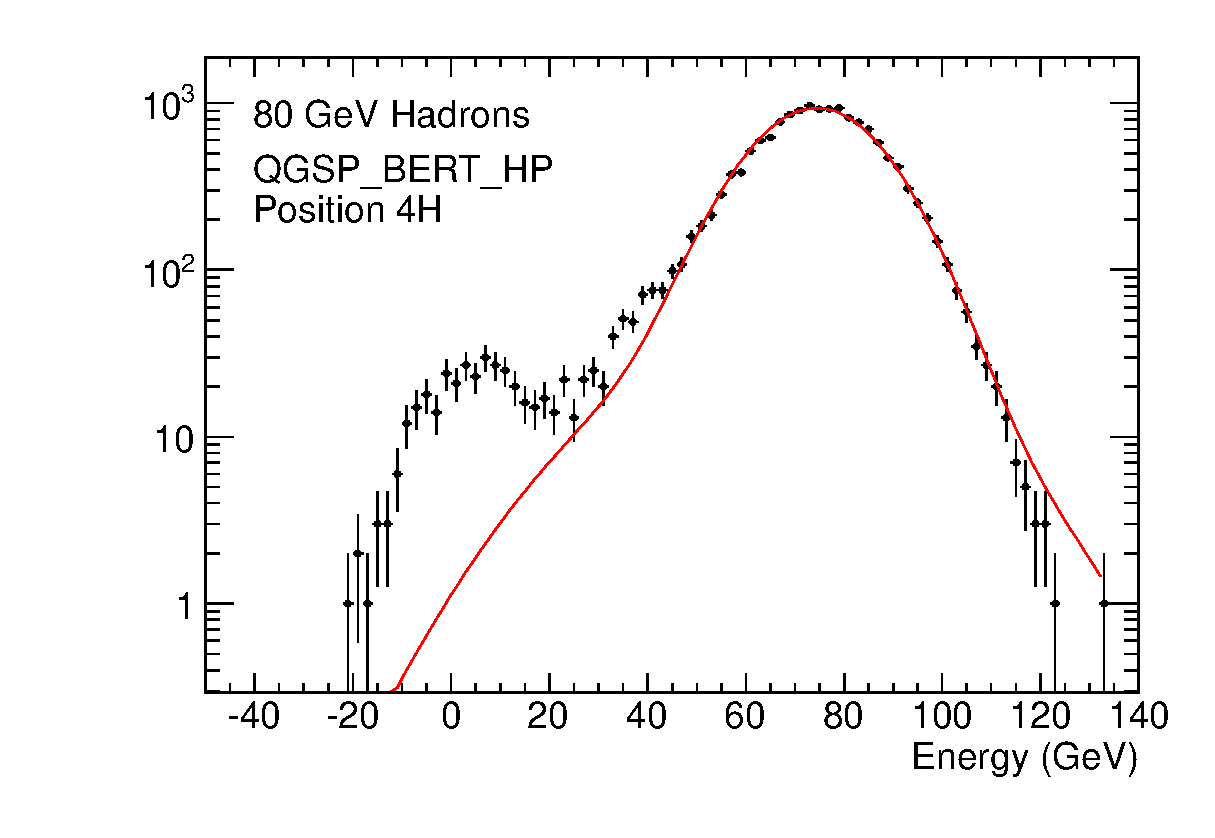
\includegraphics[width=0.45\linewidth,angle=0]{FCalTB_plots/Response_individual_MC/Pion_response_4H_80GeV_MC_QGSP_HP.eps}}
\subfigure{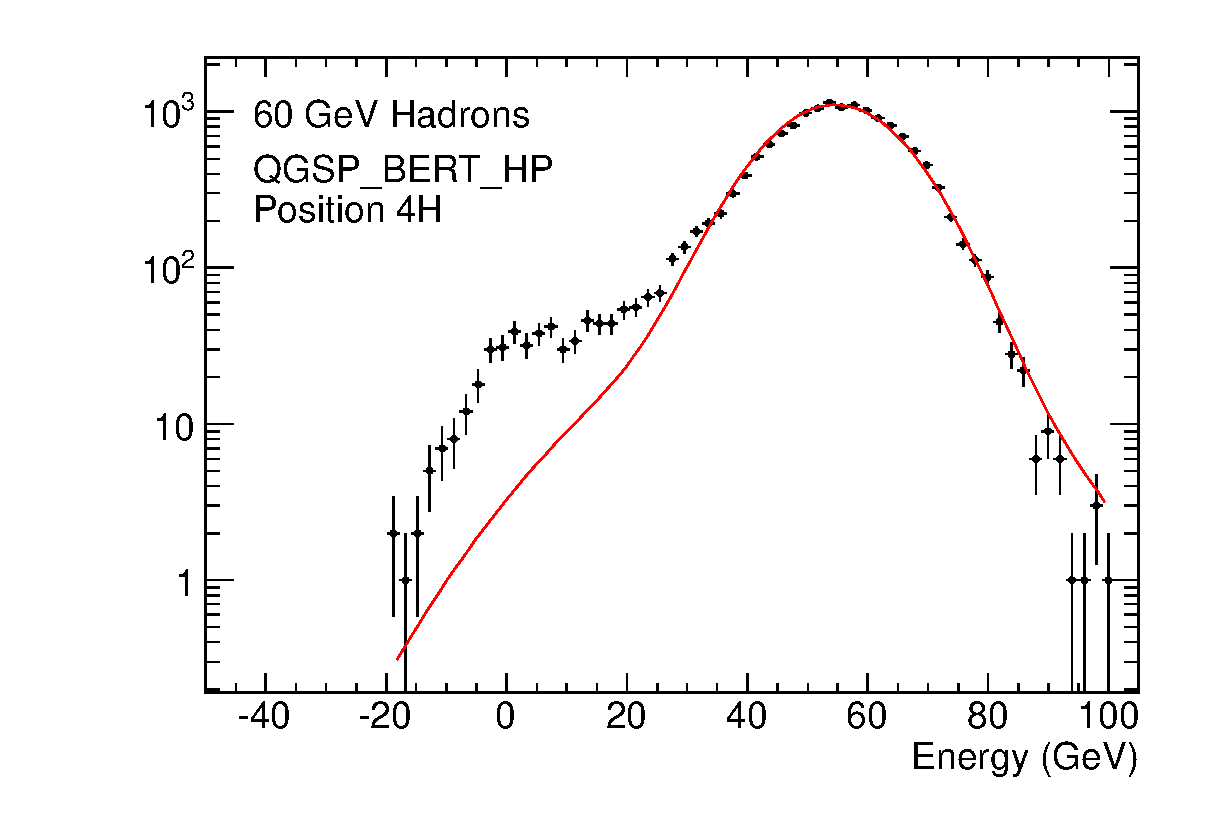
\includegraphics[width=0.45\linewidth,angle=0]{FCalTB_plots/Response_individual_MC/Pion_response_4H_60GeV_MC_QGSP_HP.eps}}\\
\subfigure{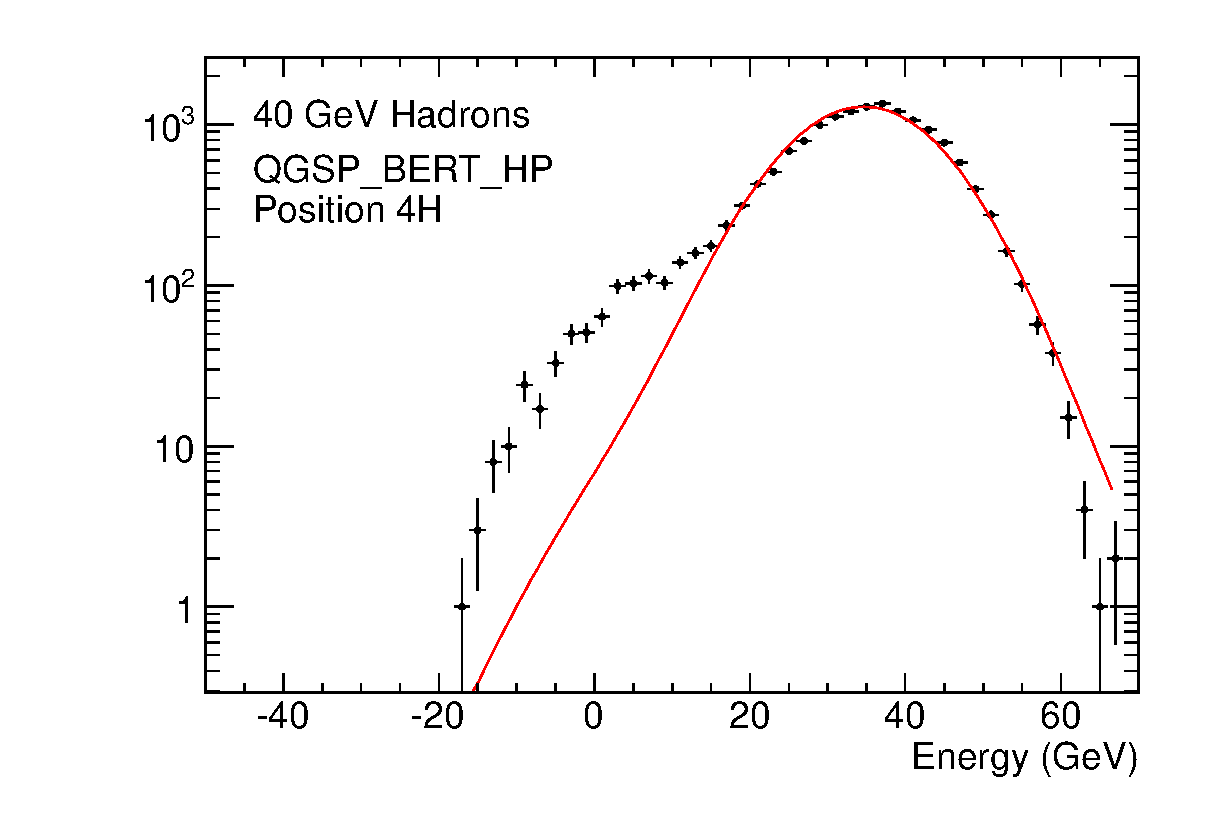
\includegraphics[width=0.45\linewidth,angle=0]{FCalTB_plots/Response_individual_MC/Pion_response_4H_40GeV_MC_QGSP_HP.eps}}
\subfigure{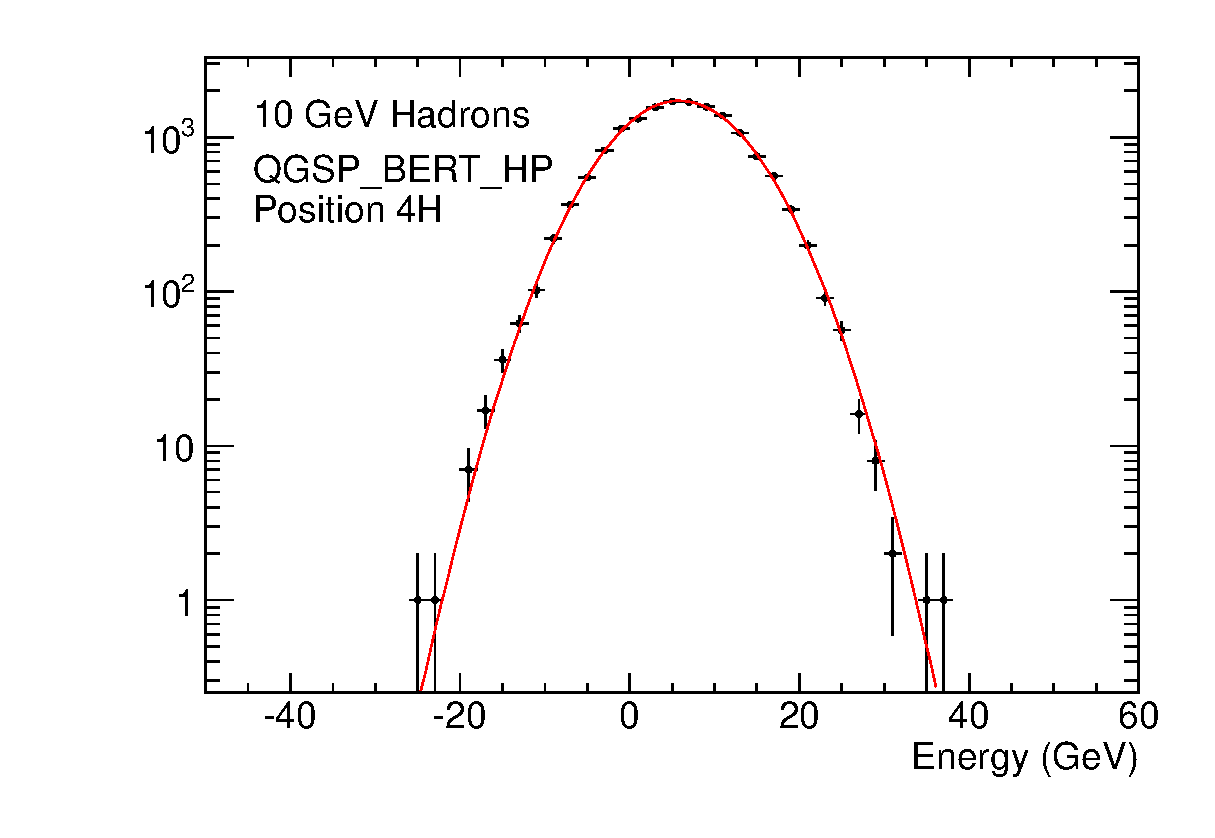
\includegraphics[width=0.45\linewidth,angle=0]{FCalTB_plots/Response_individual_MC/Pion_response_4H_10GeV_MC_QGSP_HP.eps}}\\
\end{center}
\caption[Pions at 4H, QGSP\_BERT\_HP]{Response plots for pions directed at position 4H, simulated using the QGSP\_BERT\_HP physics list.}
\label{TBplot_pion_response_4H_MC_QGSPHP}
\end{figure}


\begin{figure}[p]
\begin{center}
\subfigure{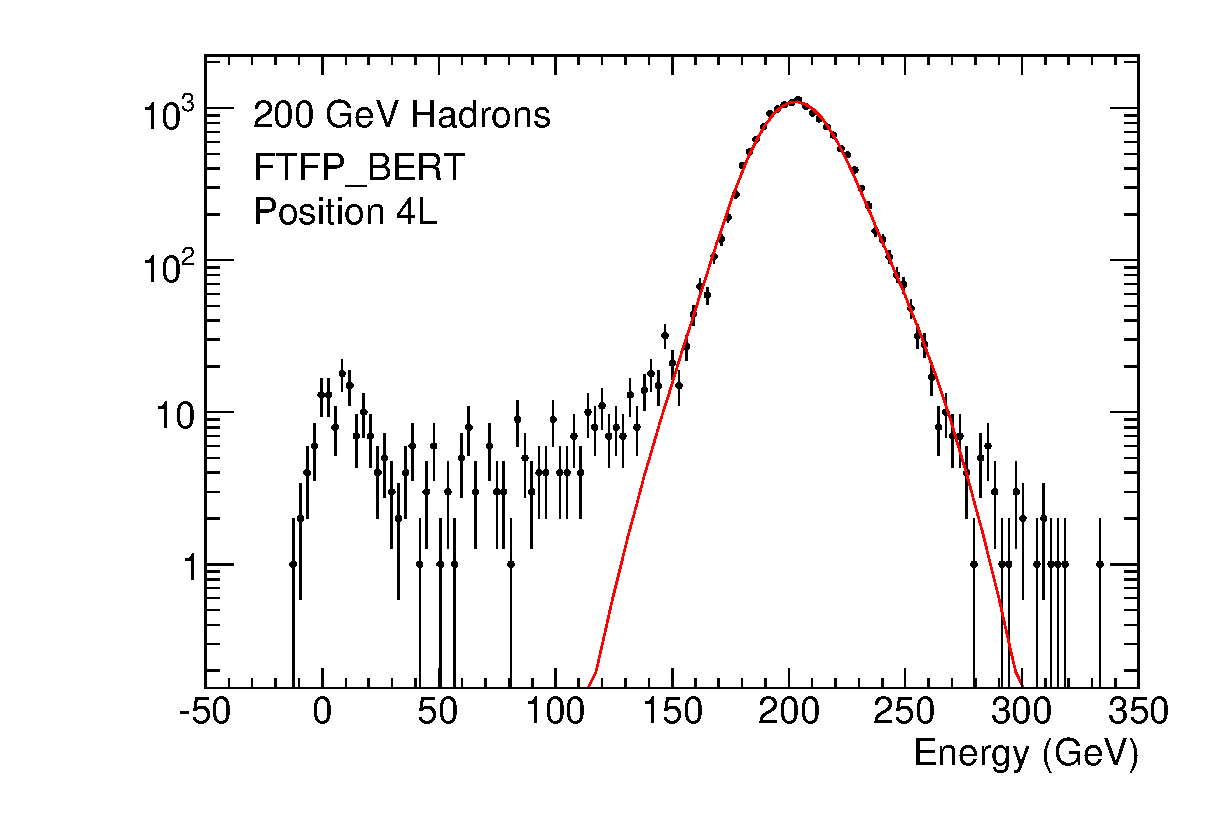
\includegraphics[width=0.45\linewidth,angle=0]{FCalTB_plots/Response_individual_MC/Pion_response_4L_200GeV_MC_FTFP.eps}}
\subfigure{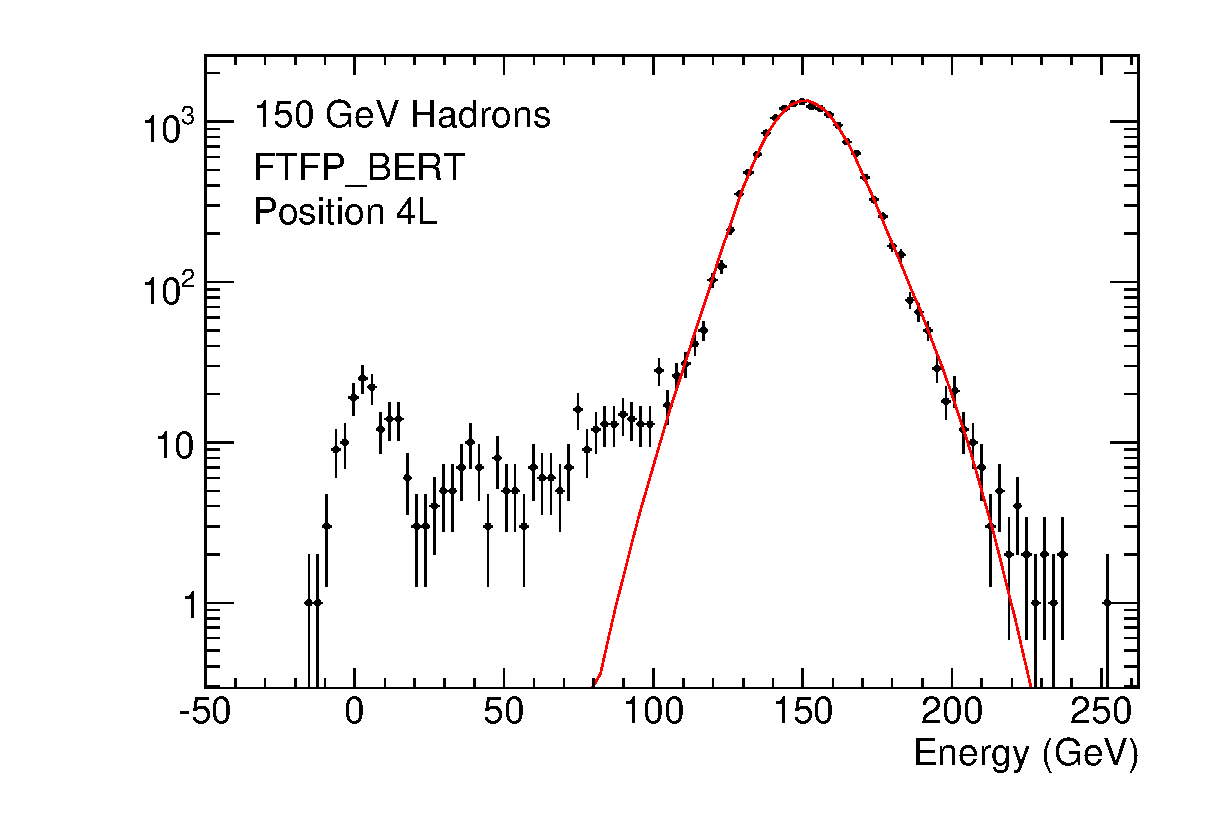
\includegraphics[width=0.45\linewidth,angle=0]{FCalTB_plots/Response_individual_MC/Pion_response_4L_150GeV_MC_FTFP.eps}}\\
\subfigure{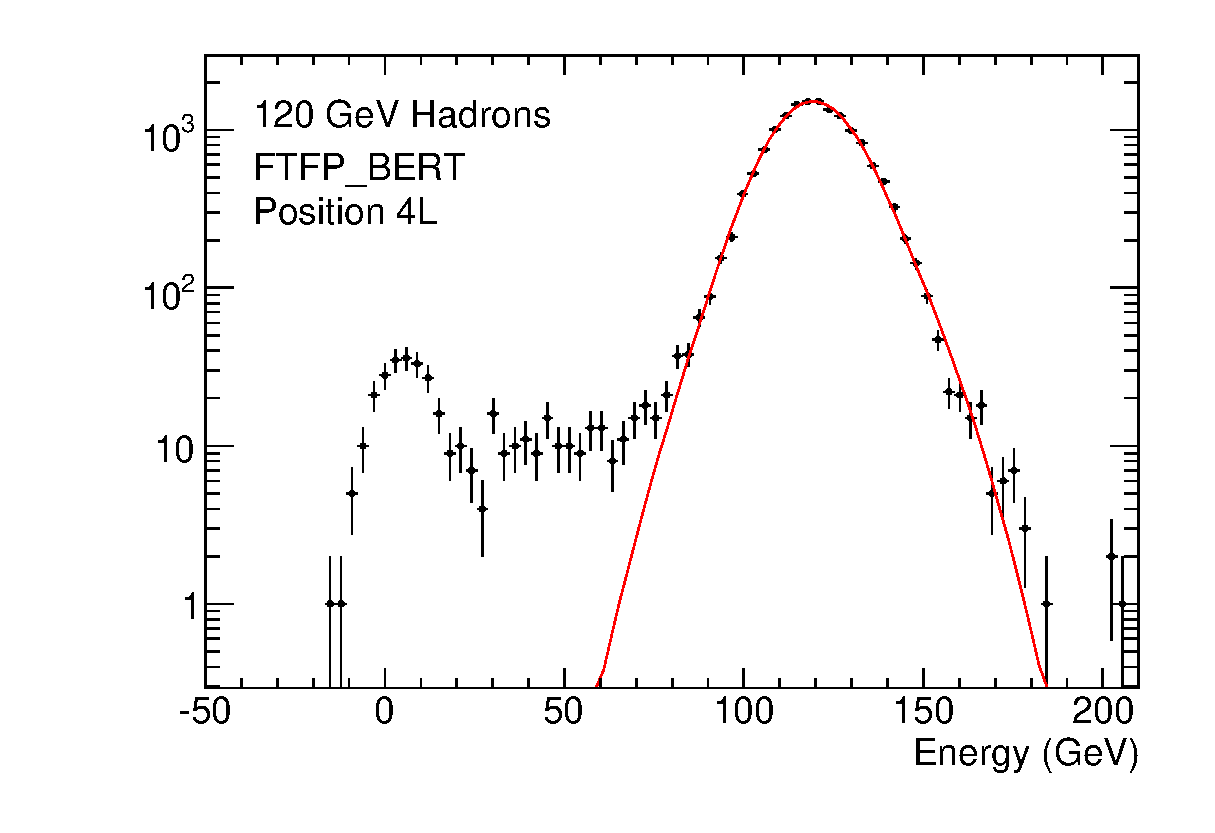
\includegraphics[width=0.45\linewidth,angle=0]{FCalTB_plots/Response_individual_MC/Pion_response_4L_120GeV_MC_FTFP.eps}}
\subfigure{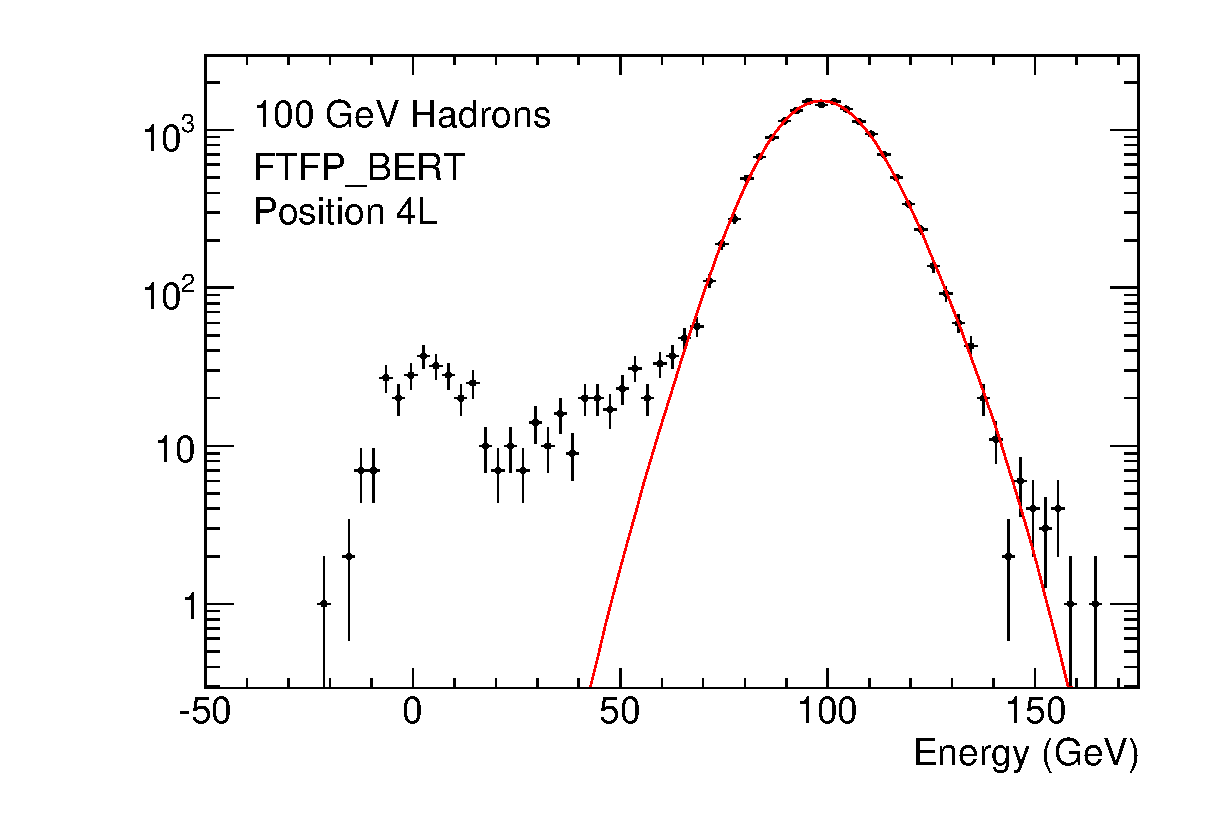
\includegraphics[width=0.45\linewidth,angle=0]{FCalTB_plots/Response_individual_MC/Pion_response_4L_100GeV_MC_FTFP.eps}}\\
\subfigure{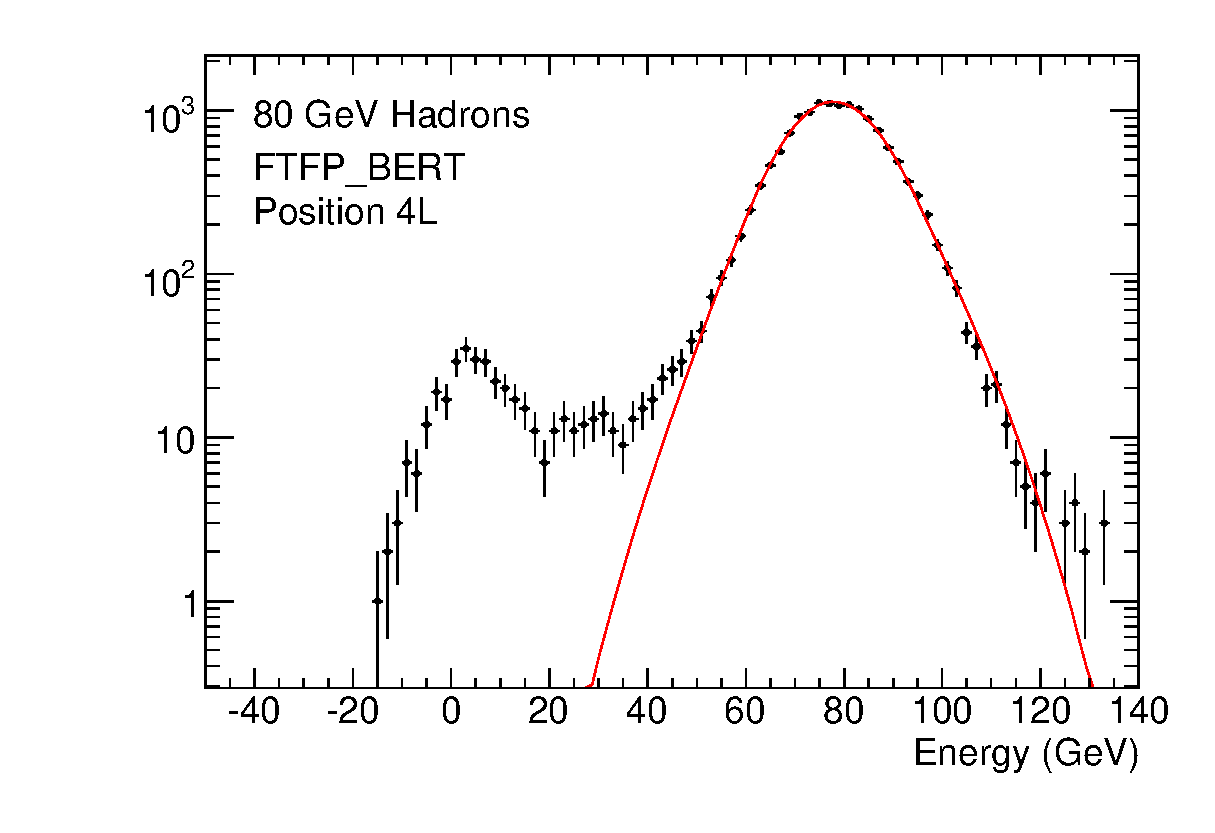
\includegraphics[width=0.45\linewidth,angle=0]{FCalTB_plots/Response_individual_MC/Pion_response_4L_80GeV_MC_FTFP.eps}}
\subfigure{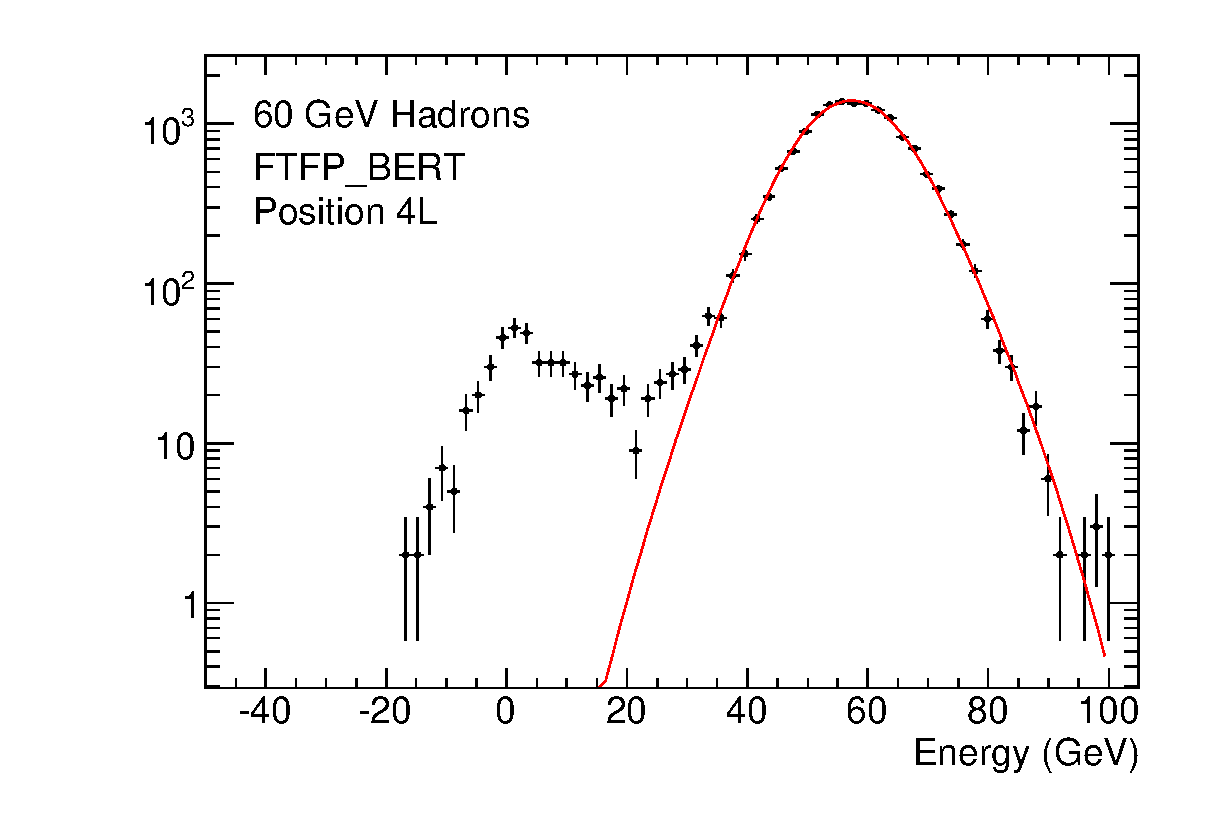
\includegraphics[width=0.45\linewidth,angle=0]{FCalTB_plots/Response_individual_MC/Pion_response_4L_60GeV_MC_FTFP.eps}}\\
\subfigure{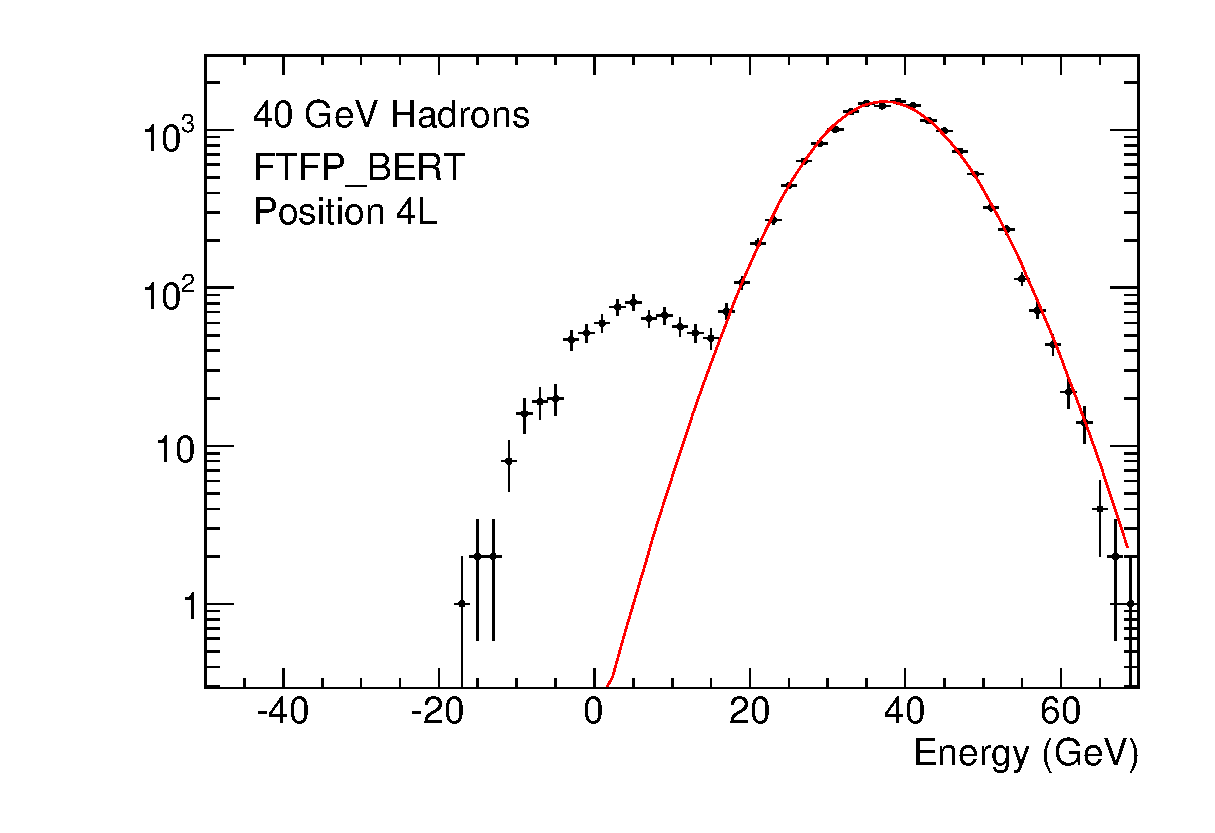
\includegraphics[width=0.45\linewidth,angle=0]{FCalTB_plots/Response_individual_MC/Pion_response_4L_40GeV_MC_FTFP.eps}}
\subfigure{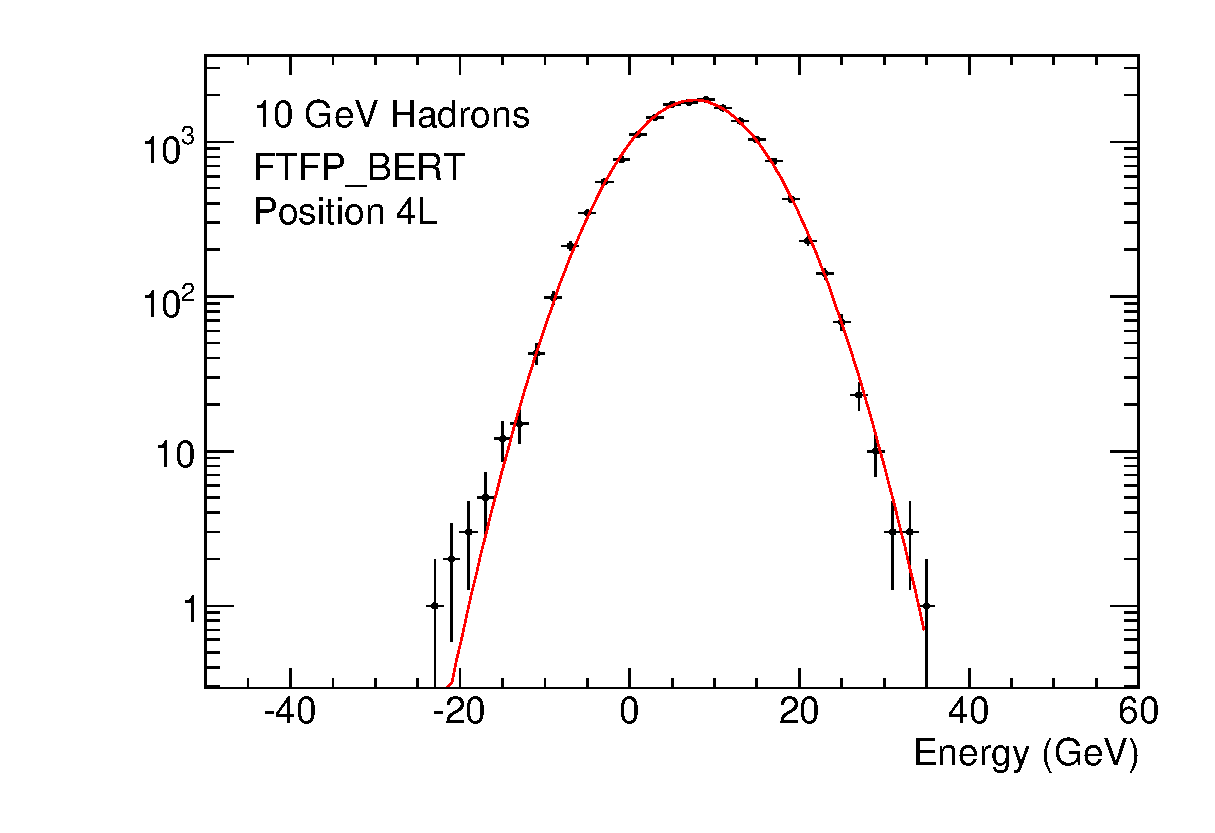
\includegraphics[width=0.45\linewidth,angle=0]{FCalTB_plots/Response_individual_MC/Pion_response_4L_10GeV_MC_FTFP.eps}}\\
\end{center}
\caption[Pions at 4L, FTFP\_BERT]{Response plots for pions directed at position 4L, simulated using the FTFP\_BERT physics list.}
\label{TBplot_pion_response_4L_MC_FTFP}
\end{figure}

\begin{figure}[p]
\begin{center}
\subfigure{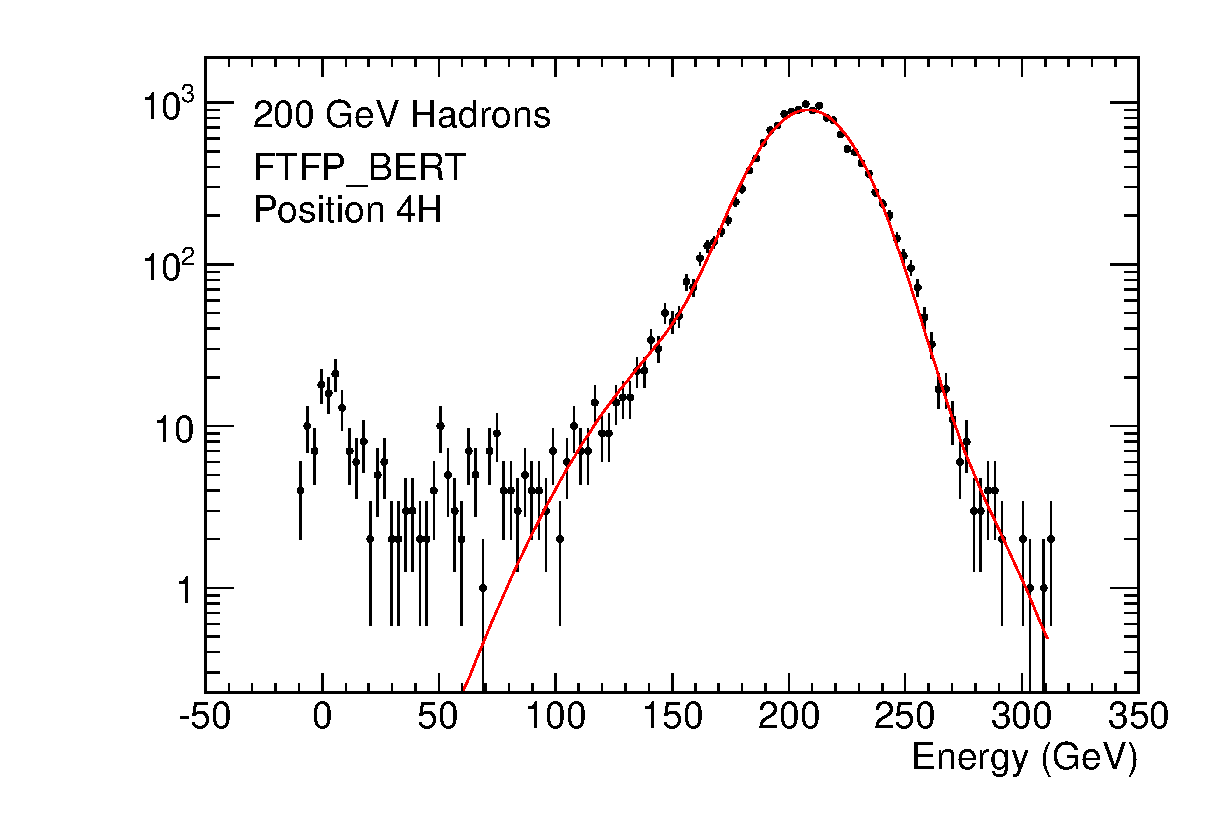
\includegraphics[width=0.45\linewidth,angle=0]{FCalTB_plots/Response_individual_MC/Pion_response_4H_200GeV_MC_FTFP.eps}}
\subfigure{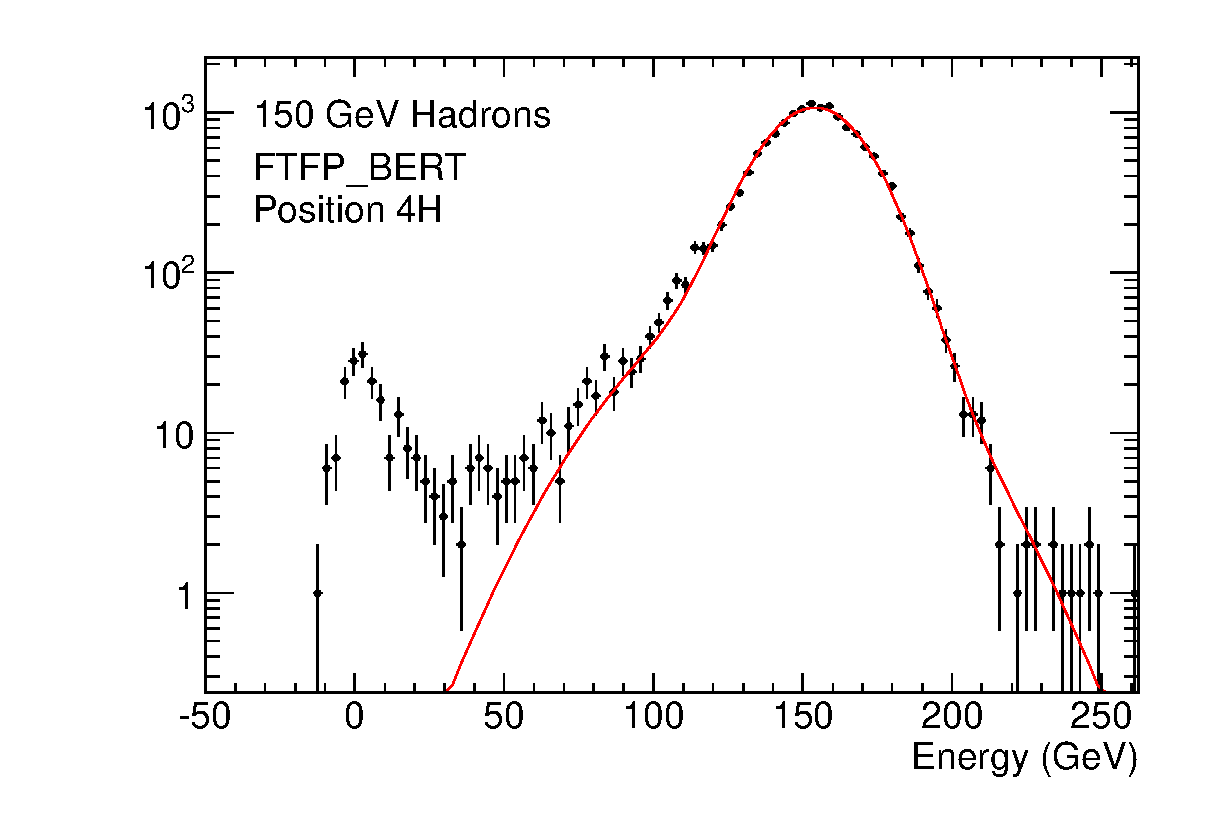
\includegraphics[width=0.45\linewidth,angle=0]{FCalTB_plots/Response_individual_MC/Pion_response_4H_150GeV_MC_FTFP.eps}}\\
\subfigure{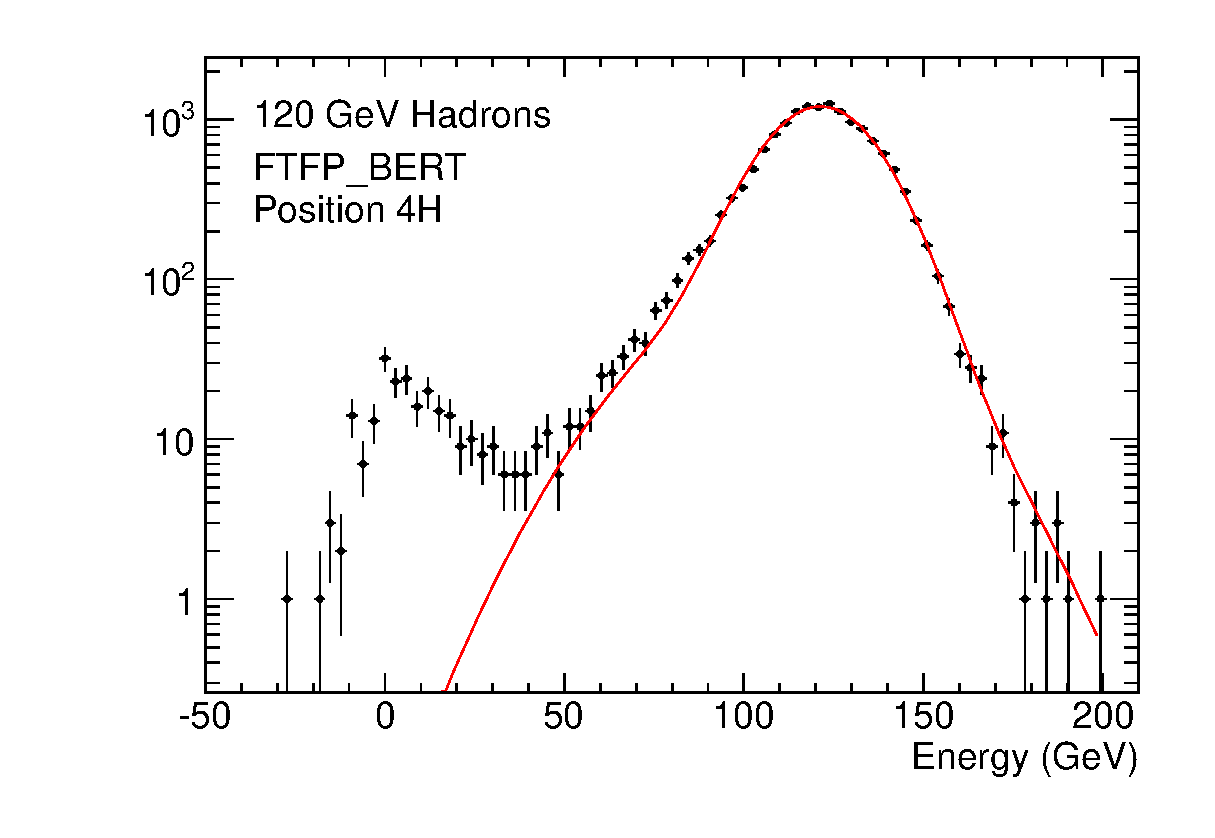
\includegraphics[width=0.45\linewidth,angle=0]{FCalTB_plots/Response_individual_MC/Pion_response_4H_120GeV_MC_FTFP.eps}}
\subfigure{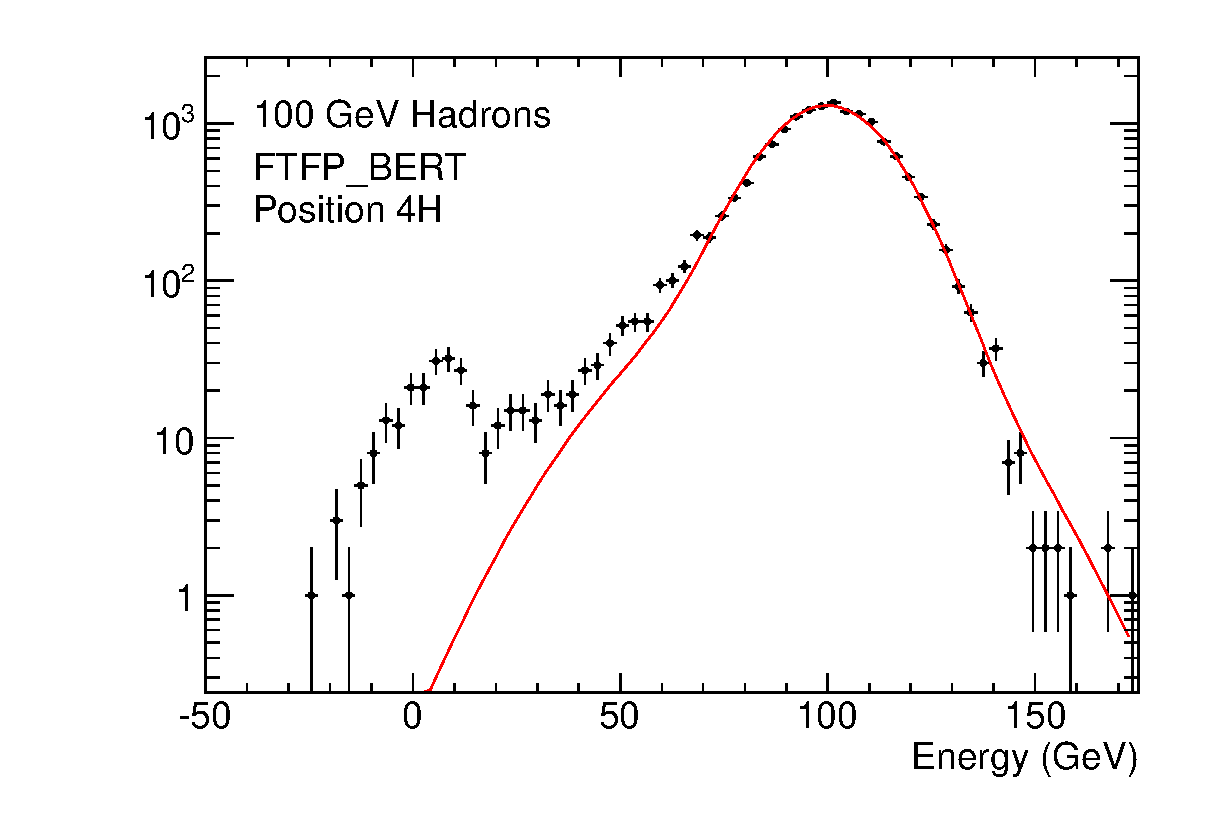
\includegraphics[width=0.45\linewidth,angle=0]{FCalTB_plots/Response_individual_MC/Pion_response_4H_100GeV_MC_FTFP.eps}}\\
\subfigure{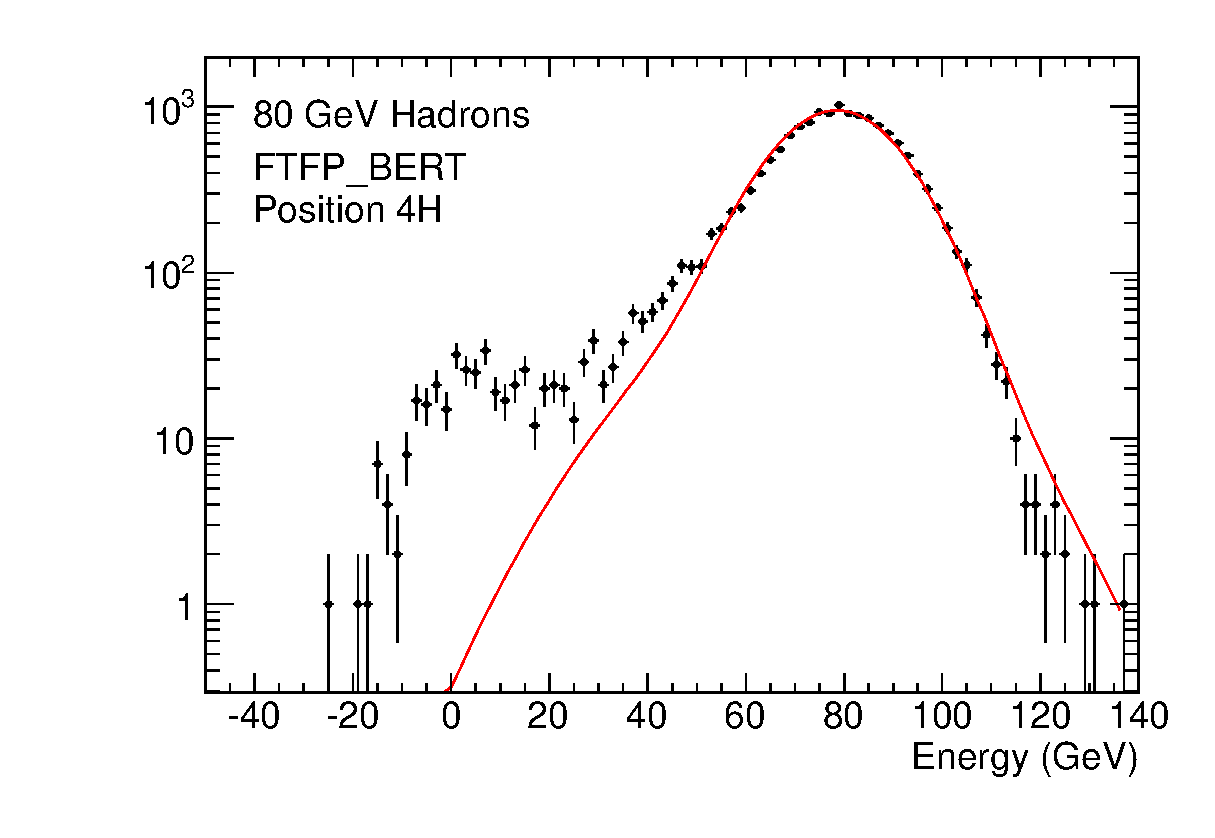
\includegraphics[width=0.45\linewidth,angle=0]{FCalTB_plots/Response_individual_MC/Pion_response_4H_80GeV_MC_FTFP.eps}}
\subfigure{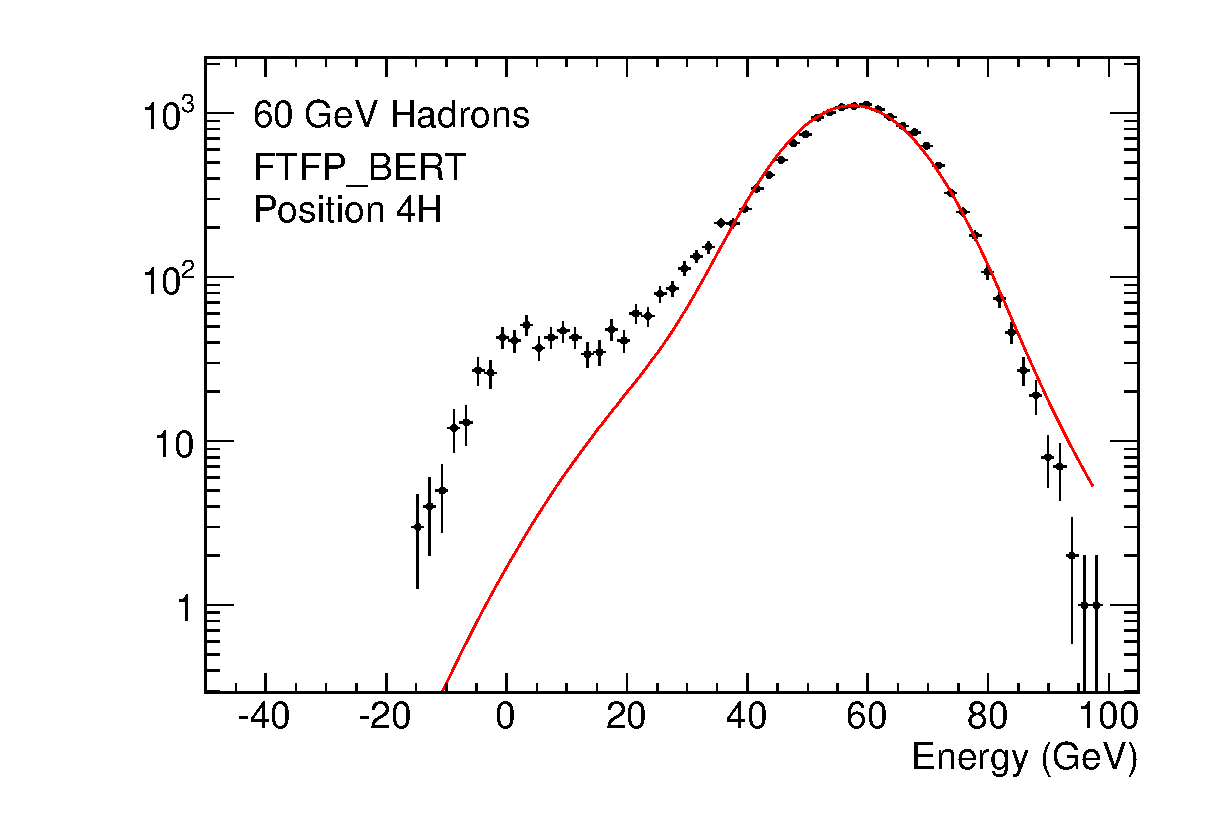
\includegraphics[width=0.45\linewidth,angle=0]{FCalTB_plots/Response_individual_MC/Pion_response_4H_60GeV_MC_FTFP.eps}}\\
\subfigure{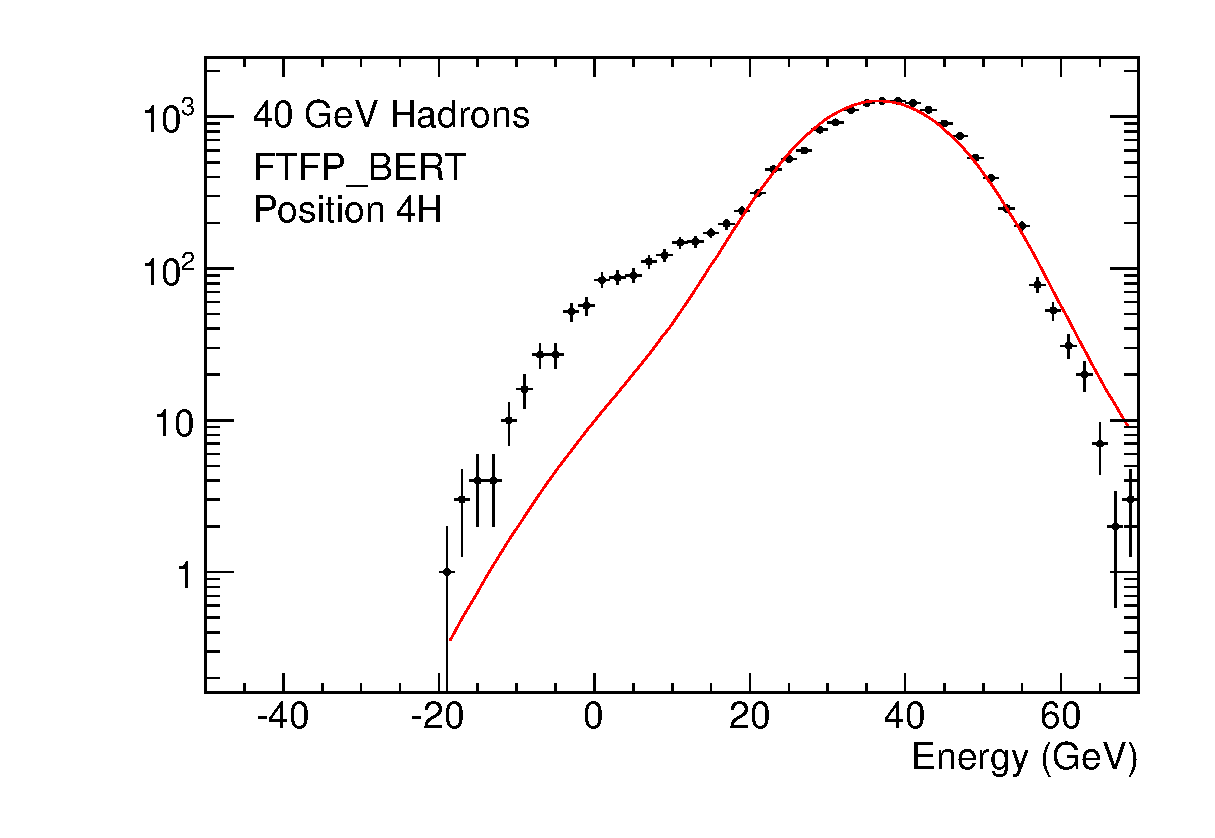
\includegraphics[width=0.45\linewidth,angle=0]{FCalTB_plots/Response_individual_MC/Pion_response_4H_40GeV_MC_FTFP.eps}}
\subfigure{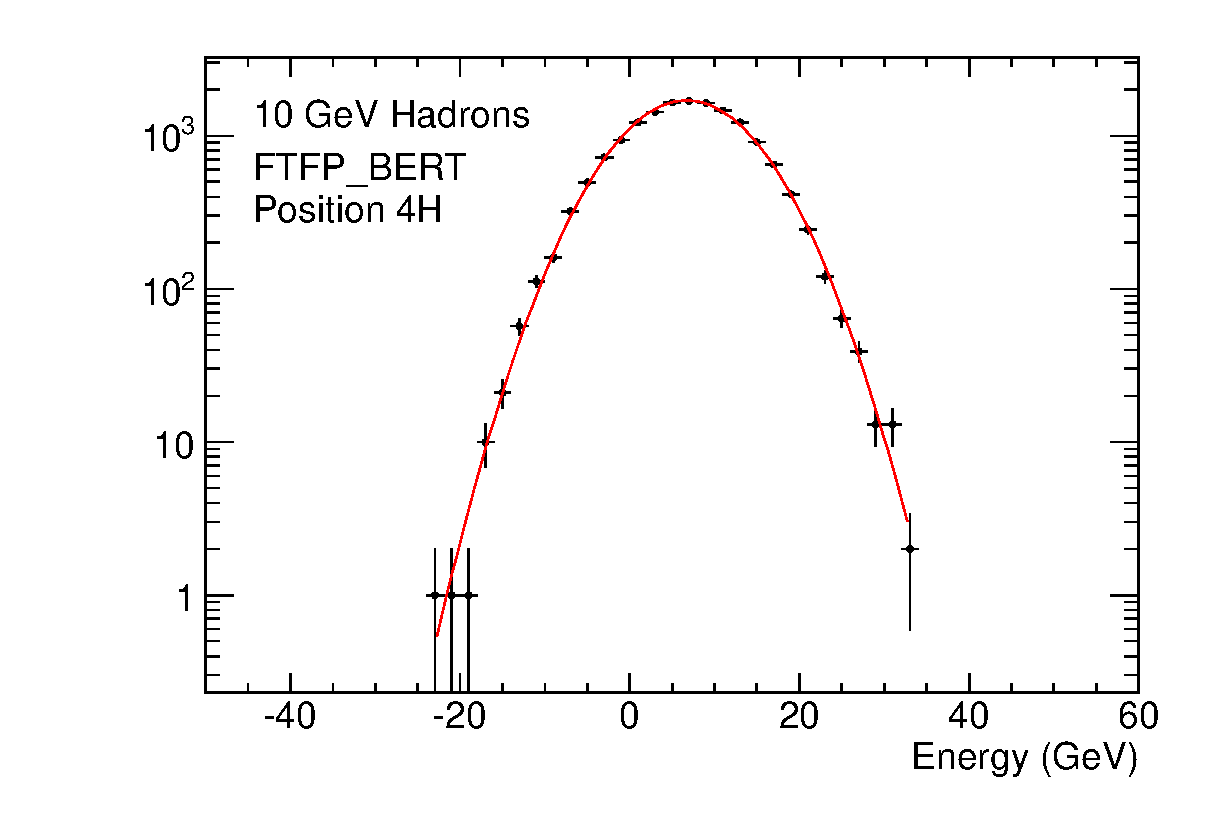
\includegraphics[width=0.45\linewidth,angle=0]{FCalTB_plots/Response_individual_MC/Pion_response_4H_10GeV_MC_FTFP.eps}}\\
\end{center}
\caption[Pions at 4H, FTFP\_BERT]{Response plots for pions directed at position 4H, simulated using the FTFP\_BERT physics list.}
\label{TBplot_pion_response_4H_MC_FTFP}
\end{figure}

\clearpage
\section{Results Obtained using Topological Clusters}
Figures~\ref{TBplot_pion_response_4L_MC_QGSP_t420} (\ref{TBplot_pion_response_4H_MC_QGSP_t420}), \ref{TBplot_pion_response_4L_MC_QGSPHP_t420} (\ref{TBplot_pion_response_4H_MC_QGSPHP_t420}), and \ref{TBplot_pion_response_4L_MC_FTFP_t420} (\ref{TBplot_pion_response_4H_MC_FTFP_t420}) show the responses obtained from beams of pions directed at position 4L (4H), for the QGSP\_BERT, QGSP\_BERT\_HP, and FTFP\_BERT physics lists, respectively. The results presented here are obtained using a topological clustering method, with ``420'' thresholds. Hadronic calibration is again carried out using the flat-weighting method, with the weights derived from 200 GeV data.








\begin{figure}[p]
\begin{center}
\subfigure{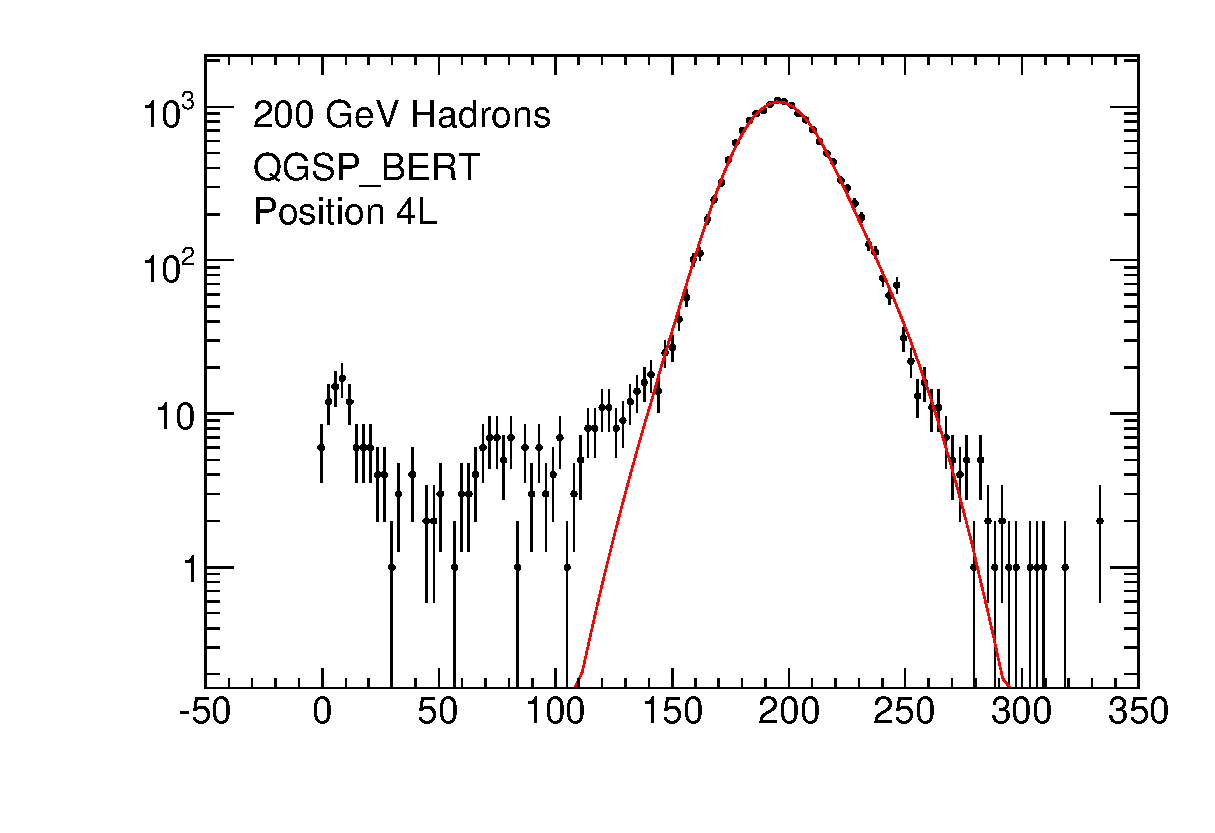
\includegraphics[width=0.45\linewidth,angle=0]{FCalTB_plots/Response_individual_MC/Pion_response_4L_200GeV_MC_QGSP_t420.eps}}
\subfigure{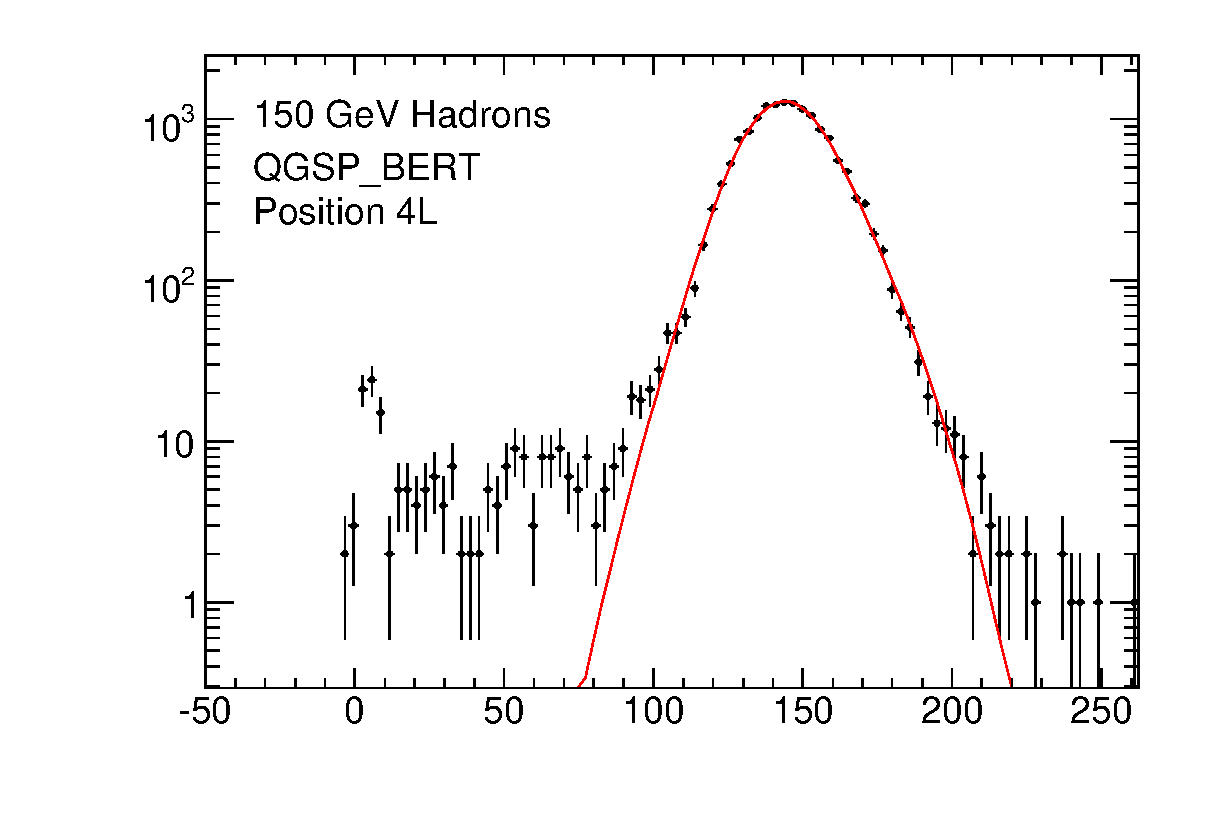
\includegraphics[width=0.45\linewidth,angle=0]{FCalTB_plots/Response_individual_MC/Pion_response_4L_150GeV_MC_QGSP_t420.eps}}\\
\subfigure{\includegraphics[width=0.45\linewidth,angle=0]{FCalTB_plots/Response_individual_MC/Pion_response_4L_120GeV_MC_QGSP_t420.eps}}
\subfigure{\includegraphics[width=0.45\linewidth,angle=0]{FCalTB_plots/Response_individual_MC/Pion_response_4L_100GeV_MC_QGSP_t420.eps}}\\
\subfigure{\includegraphics[width=0.45\linewidth,angle=0]{FCalTB_plots/Response_individual_MC/Pion_response_4L_80GeV_MC_QGSP_t420.eps}}
\subfigure{\includegraphics[width=0.45\linewidth,angle=0]{FCalTB_plots/Response_individual_MC/Pion_response_4L_60GeV_MC_QGSP_t420.eps}}\\
\subfigure{\includegraphics[width=0.45\linewidth,angle=0]{FCalTB_plots/Response_individual_MC/Pion_response_4L_40GeV_MC_QGSP_t420.eps}}
\subfigure{\includegraphics[width=0.45\linewidth,angle=0]{FCalTB_plots/Response_individual_MC/Pion_response_4L_10GeV_MC_QGSP_t420.eps}}\\
\end{center}
\caption[Pions at 4L, QGSP\_BERT, topoclusters]{Response plots for pions directed at position 4L, simulated using the QGSP\_BERT physics list. }
\label{TBplot_pion_response_4L_MC_QGSP_t420}
\end{figure}

\begin{figure}[p]
\begin{center}
\subfigure{\includegraphics[width=0.45\linewidth,angle=0]{FCalTB_plots/Response_individual_MC/Pion_response_4H_200GeV_MC_QGSP_t420.eps}}
\subfigure{\includegraphics[width=0.45\linewidth,angle=0]{FCalTB_plots/Response_individual_MC/Pion_response_4H_150GeV_MC_QGSP_t420.eps}}\\
\subfigure{\includegraphics[width=0.45\linewidth,angle=0]{FCalTB_plots/Response_individual_MC/Pion_response_4H_120GeV_MC_QGSP_t420.eps}}
\subfigure{\includegraphics[width=0.45\linewidth,angle=0]{FCalTB_plots/Response_individual_MC/Pion_response_4H_100GeV_MC_QGSP_t420.eps}}\\
\subfigure{\includegraphics[width=0.45\linewidth,angle=0]{FCalTB_plots/Response_individual_MC/Pion_response_4H_80GeV_MC_QGSP_t420.eps}}
\subfigure{\includegraphics[width=0.45\linewidth,angle=0]{FCalTB_plots/Response_individual_MC/Pion_response_4H_60GeV_MC_QGSP_t420.eps}}\\
\subfigure{\includegraphics[width=0.45\linewidth,angle=0]{FCalTB_plots/Response_individual_MC/Pion_response_4H_40GeV_MC_QGSP_t420.eps}}
\subfigure{\includegraphics[width=0.45\linewidth,angle=0]{FCalTB_plots/Response_individual_MC/Pion_response_4H_10GeV_MC_QGSP_t420.eps}}\\
\end{center}
\caption[Pions at 4H, QGSP\_BERT, topoclusters]{Response plots for pions directed at position 4H, simulated using the QGSP\_BERT physics list.}
\label{TBplot_pion_response_4H_MC_QGSP_t420}
\end{figure}

\begin{figure}[p]
\begin{center}
\subfigure{\includegraphics[width=0.45\linewidth,angle=0]{FCalTB_plots/Response_individual_MC/Pion_response_4L_200GeV_MC_QGSP_HP_t420.eps}}
\subfigure{\includegraphics[width=0.45\linewidth,angle=0]{FCalTB_plots/Response_individual_MC/Pion_response_4L_150GeV_MC_QGSP_HP_t420.eps}}\\
\subfigure{\includegraphics[width=0.45\linewidth,angle=0]{FCalTB_plots/Response_individual_MC/Pion_response_4L_120GeV_MC_QGSP_HP_t420.eps}}
\subfigure{\includegraphics[width=0.45\linewidth,angle=0]{FCalTB_plots/Response_individual_MC/Pion_response_4L_100GeV_MC_QGSP_HP_t420.eps}}\\
\subfigure{\includegraphics[width=0.45\linewidth,angle=0]{FCalTB_plots/Response_individual_MC/Pion_response_4L_80GeV_MC_QGSP_HP_t420.eps}}
\subfigure{\includegraphics[width=0.45\linewidth,angle=0]{FCalTB_plots/Response_individual_MC/Pion_response_4L_60GeV_MC_QGSP_HP_t420.eps}}\\
\subfigure{\includegraphics[width=0.45\linewidth,angle=0]{FCalTB_plots/Response_individual_MC/Pion_response_4L_40GeV_MC_QGSP_HP_t420.eps}}
\subfigure{\includegraphics[width=0.45\linewidth,angle=0]{FCalTB_plots/Response_individual_MC/Pion_response_4L_10GeV_MC_QGSP_HP_t420.eps}}\\
\end{center}
\caption[Pions at 4L, QGSP\_BERT\_HP, topoclusters]{Response plots for pions directed at position 4L, simulated using the QGSP\_BERT\_HP physics list.}
\label{TBplot_pion_response_4L_MC_QGSPHP_t420}
\end{figure}

\begin{figure}[p]
\begin{center}
\subfigure{\includegraphics[width=0.45\linewidth,angle=0]{FCalTB_plots/Response_individual_MC/Pion_response_4H_200GeV_MC_QGSP_HP_t420.eps}}
\subfigure{\includegraphics[width=0.45\linewidth,angle=0]{FCalTB_plots/Response_individual_MC/Pion_response_4H_150GeV_MC_QGSP_HP_t420.eps}}\\
\subfigure{\includegraphics[width=0.45\linewidth,angle=0]{FCalTB_plots/Response_individual_MC/Pion_response_4H_120GeV_MC_QGSP_HP_t420.eps}}
\subfigure{\includegraphics[width=0.45\linewidth,angle=0]{FCalTB_plots/Response_individual_MC/Pion_response_4H_100GeV_MC_QGSP_HP_t420.eps}}\\
\subfigure{\includegraphics[width=0.45\linewidth,angle=0]{FCalTB_plots/Response_individual_MC/Pion_response_4H_80GeV_MC_QGSP_HP_t420.eps}}
\subfigure{\includegraphics[width=0.45\linewidth,angle=0]{FCalTB_plots/Response_individual_MC/Pion_response_4H_60GeV_MC_QGSP_HP_t420.eps}}\\
\subfigure{\includegraphics[width=0.45\linewidth,angle=0]{FCalTB_plots/Response_individual_MC/Pion_response_4H_40GeV_MC_QGSP_HP_t420.eps}}
\subfigure{\includegraphics[width=0.45\linewidth,angle=0]{FCalTB_plots/Response_individual_MC/Pion_response_4H_10GeV_MC_QGSP_HP_t420.eps}}\\
\end{center}
\caption[Pions at 4H, QGSP\_BERT\_HP, topoclusters]{Response plots for pions directed at position 4H, simulated using the QGSP\_BERT\_HP physics list.}
\label{TBplot_pion_response_4H_MC_QGSPHP_t420}
\end{figure}


\begin{figure}[p]
\begin{center}
\subfigure{\includegraphics[width=0.45\linewidth,angle=0]{FCalTB_plots/Response_individual_MC/Pion_response_4L_200GeV_MC_FTFP_t420.eps}}
\subfigure{\includegraphics[width=0.45\linewidth,angle=0]{FCalTB_plots/Response_individual_MC/Pion_response_4L_150GeV_MC_FTFP_t420.eps}}\\
\subfigure{\includegraphics[width=0.45\linewidth,angle=0]{FCalTB_plots/Response_individual_MC/Pion_response_4L_120GeV_MC_FTFP_t420.eps}}
\subfigure{\includegraphics[width=0.45\linewidth,angle=0]{FCalTB_plots/Response_individual_MC/Pion_response_4L_100GeV_MC_FTFP_t420.eps}}\\
\subfigure{\includegraphics[width=0.45\linewidth,angle=0]{FCalTB_plots/Response_individual_MC/Pion_response_4L_80GeV_MC_FTFP_t420.eps}}
\subfigure{\includegraphics[width=0.45\linewidth,angle=0]{FCalTB_plots/Response_individual_MC/Pion_response_4L_60GeV_MC_FTFP_t420.eps}}\\
\subfigure{\includegraphics[width=0.45\linewidth,angle=0]{FCalTB_plots/Response_individual_MC/Pion_response_4L_40GeV_MC_FTFP_t420.eps}}
\subfigure{\includegraphics[width=0.45\linewidth,angle=0]{FCalTB_plots/Response_individual_MC/Pion_response_4L_10GeV_MC_FTFP_t420.eps}}\\
\end{center}
\caption[Pions at 4L, FTFP\_BERT, topoclusters]{Response plots for pions directed at position 4L, simulated using the FTFP\_BERT physics list.}
\label{TBplot_pion_response_4L_MC_FTFP_t420}
\end{figure}

\begin{figure}[p]
\begin{center}
\subfigure{\includegraphics[width=0.45\linewidth,angle=0]{FCalTB_plots/Response_individual_MC/Pion_response_4H_200GeV_MC_FTFP_t420.eps}}
\subfigure{\includegraphics[width=0.45\linewidth,angle=0]{FCalTB_plots/Response_individual_MC/Pion_response_4H_150GeV_MC_FTFP_t420.eps}}\\
\subfigure{\includegraphics[width=0.45\linewidth,angle=0]{FCalTB_plots/Response_individual_MC/Pion_response_4H_120GeV_MC_FTFP_t420.eps}}
\subfigure{\includegraphics[width=0.45\linewidth,angle=0]{FCalTB_plots/Response_individual_MC/Pion_response_4H_100GeV_MC_FTFP_t420.eps}}\\
\subfigure{\includegraphics[width=0.45\linewidth,angle=0]{FCalTB_plots/Response_individual_MC/Pion_response_4H_80GeV_MC_FTFP_t420.eps}}
\subfigure{\includegraphics[width=0.45\linewidth,angle=0]{FCalTB_plots/Response_individual_MC/Pion_response_4H_60GeV_MC_FTFP_t420.eps}}\\
\subfigure{\includegraphics[width=0.45\linewidth,angle=0]{FCalTB_plots/Response_individual_MC/Pion_response_4H_40GeV_MC_FTFP_t420.eps}}
\subfigure{\includegraphics[width=0.45\linewidth,angle=0]{FCalTB_plots/Response_individual_MC/Pion_response_4H_10GeV_MC_FTFP.eps}}\\
\end{center}
\caption[Pions at 4H, FTFP\_BERT, topoclusters]{Response plots for pions directed at position 4H, simulated using the FTFP\_BERT physics list.}
\label{TBplot_pion_response_4H_MC_FTFP_t420}
\end{figure}

